\documentclass[dutch, oneside]{tudelft-report}
\usepackage{cleveref}
\usepackage[dutch]{babel}
\usepackage{enumitem}
\usepackage{geometry}
\usepackage{graphicx}
\usepackage{hyperref}
\usepackage{listings}	
\usepackage{multirow}
\usepackage{natbib}
\usepackage{pdfpages}
\usepackage{siunitx}
\usepackage[utf8]{inputenc}

\usepackage{datetime}					% Used for some data-references
\usepackage{eso-pic}						% Absolute positioning, used for lines-to-track appendix and front- and backpage
\usepackage{keystroke}					% "Real" keys
\usepackage{longtable}					% Table is te groot
\usepackage{nameref}					% For displaying a sections name AND number
\usepackage{nextpage}					% Advanced nextpage commands
\usepackage{nonfloat}					% Captions for non-floating figures and tables
\usepackage[normalem]{ulem}				% Dingen dooruniten
\usepackage[nottoc]{tocbibind}				% Include Bibliography in ToC
\usepackage{pslatex}						% Times, helvetica and courier
\usepackage{soul}						% Dingen doorstrepen
\usepackage[T1]{fontenc}					% Nicer font-encoding
\usepackage{tabularx}					% Used for evenly spread tables
\usepackage{tikz}						% Voor fsm
\usepackage{verbatim}					% For comment-environment
\usepackage{xcolor}						% For adding colored text

\definecolor{comment}{RGB}{0, 15 , 117}		% Kleur blauw definiëren
\definecolor{keyword}{RGB}{165, 42, 42}		% Kleur rood definiëren
\definecolor{STD}{RGB}{46, 139, 87}			% Kleur groen definiëren

\lstdefinelanguage{VHDL}{
	morekeywords=[1]{ 					% Definiëren van keywords die blauw worden
		ALL, all, and, architecture, array,
		begin, case, component, downto,
		else, elsif, entity, end, for, if, in, is,
		library, loop, map, not, of, or, others,
		out, port, process, signal, then,
		to, type, use, when
},
	morekeywords=[2]{					% Definiëren van keywords die groen worden
    		NUMERIC_STD, numeric_std,
		STD_LOGIC_1164, std_logic_1164,
		STD_LOGIC_ARITH, std_logic_arith,
		STD_LOGIC_UNSIGNED, std_logic_unsigned,
		STD_LOGIC_VECTOR, std_logic_vector,
		STD_LOGIC, std_logic,
		UNSIGNED, unsigned
},
	morecomment=[l]--
}

\lstdefinestyle{vhdl}{
  language		= VHDL,
  basicstyle   	= \footnotesize \ttfamily,
  keywordstyle 	= [1]\color{keyword}\bfseries, 	% Keywords kleuren (rood)
  keywordstyle 	= [2]\color{STD}\bfseries,		% Keywords kleuren (groen)
  commentstyle	= \color{comment},			% Comments kleuren (blauw)
  numbers		= left,					% Regel nummering
  breaklines	= true,               			% sets automatic line breaking
  tabsize		= 4                       			% sets default tabsize to 4 spaces
}

\begin{document}

\frontmatter							% To use Roman numeral page numbers (title pages and table of contents)
\title[Extreme Winterslaap Interrupter\\ Final report\\ \\ 14-01-2015]{EPO-3}
\author{Projectgroep A1}
\affiliation{Technische Universiteit Delft} 
\coverimage{cover/Lightbulb}
\makecover

\chapter{Samenvatting}
Dit is het verslag van "EPO-3" van groep A1. Hierin is te vinden hoe het project is aangepakt en uitgewerkt. Het systeem dat is ontworpen lijkt op de Wake-up Light van het bedrijf Philips. De opstakels die overwonnen moesten worden zijn het ontvangen en verwerken van het DCF-77 signaal, het aansturen van het licht, het aansturen van het geluid en het aansturen van een LCD schermpje. In het verslag is te vinden hoe al deze subsystemen zijn ontworpen en uitgewerkt. 
\tableofcontents

\mainmatter							% To use Arabic numeral page numbers (all main chapters)
\chapter{Introductie}
Epo 3 staat in het teken van het ontwerpen van een chip. Wat voor product er ontworpen gaat worden ligt aan de projectgroep. Het bedenken van het ontwerp is de eerste stap in het ontwerpproces, bij deze stap moet er al rekening gehouden met de randvoorwaarden die aan het project gesteld worden, zoals het aantal beschikbare transistoren op de chip.\\
Er is besloten om een wake-up light te maken. De belangrijkste functie is dat het licht 15 minuten voor de alarmtijd langzaam aan begint te gaan, totdat de lamp op de alarmtijd op volle sterkte brandt. Daarnaast zullen er nog een paar functies toegevoegd worden. Het DCF-signaal zal opgevangen worden voor de actuele datum en tijd, dit zal op een LCD-scherm worden laten zien. Door middel van vijf knoppen kan de wekker bediend worden. De alarmtijd kan ingesteld worden en de gebruiker kan aangeven of het licht en geluid aan moeten gaan als de gebruiker gewekt wil worden. Op de LCD zal ook te zien zijn of er iets aangepast wordt. De ingangs- en uitgangssignalen en het gedrag moeten geformuleerd worden als specificaties.\\
Er wordt structuur aangebracht in het systeem door het systeem op te delen in een paar grote blokken, deze blokken kunnen dan over de acht projectleden verdeeld worden. Allereerst moeten er van de afzonderlijke subsystemen specificaties opgesteld worden, zodat de blokken op elkaar afgestemd kunnen worden. Vervolgens moet van elk blok \'e\'en of meer FSM's gemaakt worden waarna er een code geschreven kan worden. De geschreven code moet gesimuleerd en gesyntetiseerd worden. Als aan het eind van het project van het hele systeem een lay-out gemaakt is, kan het systeem op een chip gezet worden.

\chapter{Ontwerp specificatie}
% korte beschrijving wat de schakeling moet doen
Voor ons project ontwerpen we een klok, gesynchroniseerd met DCF77, weergeven op lcd met een wake-up alarm. De tijd, die intern wordt bijgehouden, zal worden gesynchroniseerd met een zogenaamd DCF signaal. De wekker zal bediend worden door middel van een menu. Dit menu wordt aangestuurd op basis van 4 knoppen. In dit menu moet de wekkertijd ingesteld worden. Ook moet de wekker en het wekkergeluid aan en uit gezet kunnen worden. Een vijfde knop is de uitknop voor als de wekker gaat en uitgezet moet worden. De visualisatie van dit menu zal op een LCD weergegeven worden. Als men zich niet in het menu bevindt, zal men alle data verdeeld over het scherm zien. Deze data bestaat uit de actuele tijd, de wekkertijd, de datum en de weekdag. Daarnaast zal op het LCD-scherm weergegeven worden of de wekker en het geluid aan staan. Met het knipperen van scheidingsteken tussen uren en minuten zal het passeren van seconden aangegeven worden.\\

% randvoorwaarden vastellen 
\noindent Het systeem zal enkele reandvoorwaarden hebben. Zo zal het een algemene reset moeten bevatten. Als gevolg van het indrukken van een resetknop zullen alle opgeslagen waarden en counters op 'nul' worden gezet. Ook zullen alle signalen 'active high' moeten zijn. De implementatie van het totale ontwerp moet op een chip-oppervlak van circa 0.4 cm\textsuperscript{2}, oftewel 40.000 transistor-paren. Dit in de vorm van twee opeengestapelde bond\_bars, zoals aangelevert door de TU Delft. De chip beschikt over 32 pins voor i/o poorten. Daar zitten niet de voedingspinnen bij, deze worden apart aangesloten. Voor de FSM’s (Finite State Machine) mogen alleen die van het Moore-type gebruikt worden. Als de schakeling geactiveerd wordt moeten alle FSM’s in hun begintoestand komen door middel van een reset signaal. Voor de opwekking van het kloksignaal kan gebruik gemaakt worden van een kristal van 6.144 MHz of 32 kHz. Het streven is om zo weinig mogelijk componenten extern te gebruiken. De dissipatie van de chip dient echter ook beperkt te zijn. Dit geeft een compromis voor de maximale stroom die de elektronica mag dissiperen voor de aansturing van externe componenten, zoals LEDs. De voedingsspanning van het IC bedraagt 5 Volt. Het IC wordt gemaakt in een semi-custom CMOS proces. ~\cite{handleiding}\\

Het systeem zal de volgende ingangen hebben:
\begin{itemize}[nolistsep]
\item	DCF-signaal
\item	36kHz klok
\item	Reset-knop
\item	4 menu-knoppen
\item  1 uit-knop
\end{itemize}

\noindent
\\
Onze chip zal over de volgende uitgangen beschikken:
\begin{itemize}[nolistsep]
\item	LED, 1 bit om de led aan te sturen
\item	Sound, 1 bit om de buzzer aan te sturen
\item	LCD, een 7 bits vector om het scherm aan te sturen via een microcontroller
\item  Clk\_out, 1 bit ter aansturing van de microcontroller
\end{itemize}

\chapter{Systeem overzicht en ontwerp}
Het systeem is opgedeeld in vier blokken:
\begin{itemize}
\item De DCF controller
\item De main controller
\item Het alarm
\item De LCD controller
\end{itemize}

\noindent In figuur \ref{fig:Blokdiagram} is te zien welke ingangs- en uitgangssignalen het systeem in en uit gaan en hoe de blokken elkaar aansturen.

\begin{figure}[h!]
\center
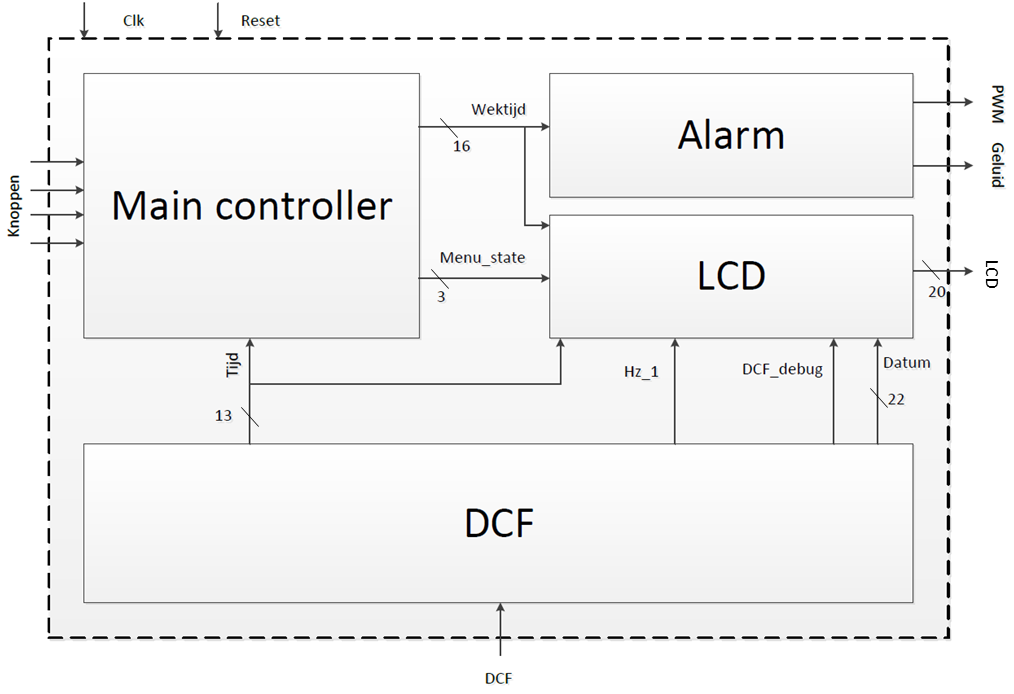
\includegraphics[width=15cm]{Figuren/Blokdiagram}
\caption{Blokdiagram van het gehele systeem}
\label{fig:Blokdiagram}
\end{figure}

\noindent In de DCF controller wordt het DCF signaal opgevangen en omgezet naar een bitvector met weekdag, datum en tijd. Daarnaast wordt er een kloksignaal van 1 Hz gegenereerd. Mocht het DCF-signaal tijdelijk niet goed opgevangen kunnen worden, kan een intern register de tijd door blijven geven en op de LCD wordt aangegeven of het DCF signaal opgevangen wordt. Dit register wordt dan weer gesynchroniseerd als het signaal weer opgevangen wordt.\\
De main controller bestuurt het hele systeem. De alarmtijd kan ingesteld worden en de alarmtijd wordt met de actuele tijd vergeleken, zodat het alarmblok weet wanneer het alarm aan moet gaan. Met knoppen kan het menu bediend worden.\\
In het alarmblok wordt eerst de vijftien minuten van de wekkertijd afgetrokken. De ingestelde tijd is namelijk de tijd waarop het geluid aan moet gaan, de lamp moet al een kwartier eerder beginnen met branden. Daarnaast zorgt het alarm ervoor dat een PWM-signaal gegenereerd wordt wat naar een LED gaat. \\
De LCD controller zorgt dat de datum, tijd, ingestelde alarmtijd en de veranderingen in het menu op de LCD zichtbaar zijn. Er wordt een LCD scherm gebruikt waar de pixels afzonderlijk van elkaar aangestuurd worden. Tussen de chip en het scherm zit nog een microcontroller, waarin de karakters zijn opgeslagen, dit zou namelijk te groot zijn om op de chip te regelen.


\chapter{DCF controller}
\section{Inleiding}
De basis van onze wekker wordt gelegd door een klok. Uit dit onderdeel, genaamd DCF-controller,  komt verschillende data, als de tijd, de datum en het weeknummer. Van de tijd uitgang wordt verwacht dat deze gesynchroniseerd met het DCF-signaal is, maar mocht het signaal uitvallen moet de tijd door blijven tellen.\\ \emph{\color{red} \#\# stukje over DCF77 \#\#}

\section{Specificaties}
In deze sectie zullen we de in- en uitgangen van de DCF-controller in een overzicht weergeven. Doordat het totale systeem met dit onderdeel start, bevat dit blok enkel standaard ingangen en een ingang van buitenaf. De uitgangen uren en minuten worden doorgestuurd naar de main-controller. De clk van 1 Hz zal in verschillende onderdelen worden gebruikt. De debug\_led zal rechtstreeks op het LCD worden weergegeven.
\subsection{Ingangen}
Dit onderdeel maakt gebruik van de volgende ingangen: 

\begin{itemize}[nolistsep]
\item Reset, standaard input.
\item Klok, standaard input.
\item DCF, signaal van 'logische' pulsen.
\end{itemize}
\noindent

\subsection{Uitgangen}
Dit onderdeel heeft de volgende uitgangen:
\begin{itemize}[nolistsep]
\item Uren, een BCD vector van 6 bits.
\item minuten, een BCD vector van 7 bits.
\item clk, een clk die elke seconde een puls geeft.
\item debug\_led, een signaal dat een logische 1 doorgeeft zodra er een dcf signaal wordt ontvangen.
\end{itemize}


\section{Gedrag}

Een van de eigenschappen van deze klok zal zijn dat hij gesynchroniseerd wordt met een zogenaamd DCF-signaal. Dit is een signaal dat in duitsland verzonden wordt en allerlei informatie bevat, als de actuele tijd en de datum. Wij zullen meerdere van deze elementen gebruiken in onze wekker.  Al deze data wordt verzonden door middel van een pulssignaal. Vanuit Duitland wordt elke seconde een puls van 100 of 200 ms verstuurd, zodat respectievelijk een 0-bit en een 1-bit doorgegeven wordt. Dit resulteert in een totaal van 59 bits, gevolgt door een seconde ‘rust’, dat elke minuut opnieuw verzonden wordt. De uren en minuten van dit signaal zullen gebruikt worden om de tijd van een interne klok bij te werken. Daarnaast zal de dag van de week, de dag van de maand, de maand en het jaar doorgegeven naar de andere onderdelen van de wekker doorgegeven.

\chapter{Main controller}
\section{Inleiding}
De main controller bevat de interface van de wekker. Deze zorgt er voor dat een wekker ingesteld kan worden, aangepast kan worden en uitgezet kan worden. 
Belangrijk aan elke interface is dat deze gebruiksvriendelijk is. 
Dit kan onder andere bereikt worden door een optimum voor het aantal knoppen te bepalen. 
Te veel knoppen, en de gebruiker weet niet welke knop wat doet, te weinig knoppen, en de gebruiker moet navigeren door een nodeloos ingewikkeld menu. \\
Daarnaast is er nog een beperkende factor: het aantal pinnen op de chip. \\
Al deze informatie samengenomen is besloten dat 4 knoppen voor de interface het meest gebruiksvriendelijke resultaat oplevert. Daarnaast is er nog een knop die slechts gebruikt wordt om een afgaand alarm uit te zetten. \\
De controller stuurt een hoop dingen aan, en van te voren was al geanticipeerd dat dit hierdoor een van de grootste onderdelen op de chip zou kunnen worden.

\section{Specificaties}
\subsection{Ingangen}
\begin{itemize}[nolistsep]
\item Klok, dit is een standaard input;
\item Reset, ook dit is een standaard input;
\item Knoppen, dit zijn de 4 knoppen die (nadat ze gebufferd zijn) onderdeel zijn van de interface.
\begin{itemize}[nolistsep]
\item knoppen[0] = menu
\item knoppen[1] = set 
\item knoppen[2] = up
\item knoppen[3] = down\\
\end{itemize}
\end{itemize}



\subsection{Uitgangen}
\begin{itemize}[nolistsep]
\item Wekker, dit is de tijd dat de wekker af moet gaan en de wekkerdata, dus of het licht en geluid aan staan, en of de wekker uberhaupt aanstaat;
\item Menu-state, dit is de staat in welke de FSM zich op het moment bevindt. Deze informatie wordt doorgevoerd naar het LCD-scherm om zo te kunnen zien waar in het menu men zit.\\
\end{itemize}
In \cref{tab:uitgangen_controller} staat wat voor informatie te vinden is in de uitgangen van de controller.
\begin{table}[ht!]
\caption{Uitgangen van de controller}
\label{tab:uitgangen_controller}
\begin{tabular*}{\textwidth}{@{\extracolsep{\fill} }|l| p{.75\textwidth}|}
\hline
Uitgang & Informatie over wat in de uitgang te vinden is \\ \hline
wekker & De huidige info over de wekker instellingen uit geheugen \newline
wekker[5 down to 0] daarin staan de minuten \newline
wekker[10 down to 6] daarin staan de uren \newline
wekker[11] geluid bit \newline
wekker[12] led bit \newline
wekker[13] wekker bit (Of de wekker uberhaupt aan is of niet) \\ \hline
menu & Deze geeft door aan de in welke state we zitten aan de lcd module \newline
000 : Het normale scherm weergeven met alarm en wekkertijd weergave state: Rust,Wekkertijd \newline
001 : Uren aanpassen \newline
010 : Minuten aanpassen \newline
011 : Led aanpassen \newline
100 : Geluid aanpassen \\ \hline
\end{tabular*}
\end{table}
\newpage
\subsection{Gedrag}
Om te beginnen moet de tijd waarop de wekker af moet gaan ingesteld kunnen worden. Dit wordt gedaan door eerst de huidige wekkertijd weer te geven, vervolgens het uur waarop gewekt moet worden te wijzigen en daarna de minuut. Hierna wordt de huidige tijd weer weergegeven. \\
Daarnaast is een vereiste dat de led uitgezet moet kunnen worden. Afhankelijk van een instelling moet het wake-up-light gedeelte wel of niet aangaan. Hetzelfde geld voor het geluid. \\
Dit alles moet zo gebruiksvriendelijk mogelijk gebeuren.

\section{Functionaliteit}

\subsection{FSM}
In \cref{fig:FSM_controller} staat de gemaakte fsm en in \cref{tab:states_controller} staan de uitgangen per state gespecificeerd.

\begin{figure}[ht!]
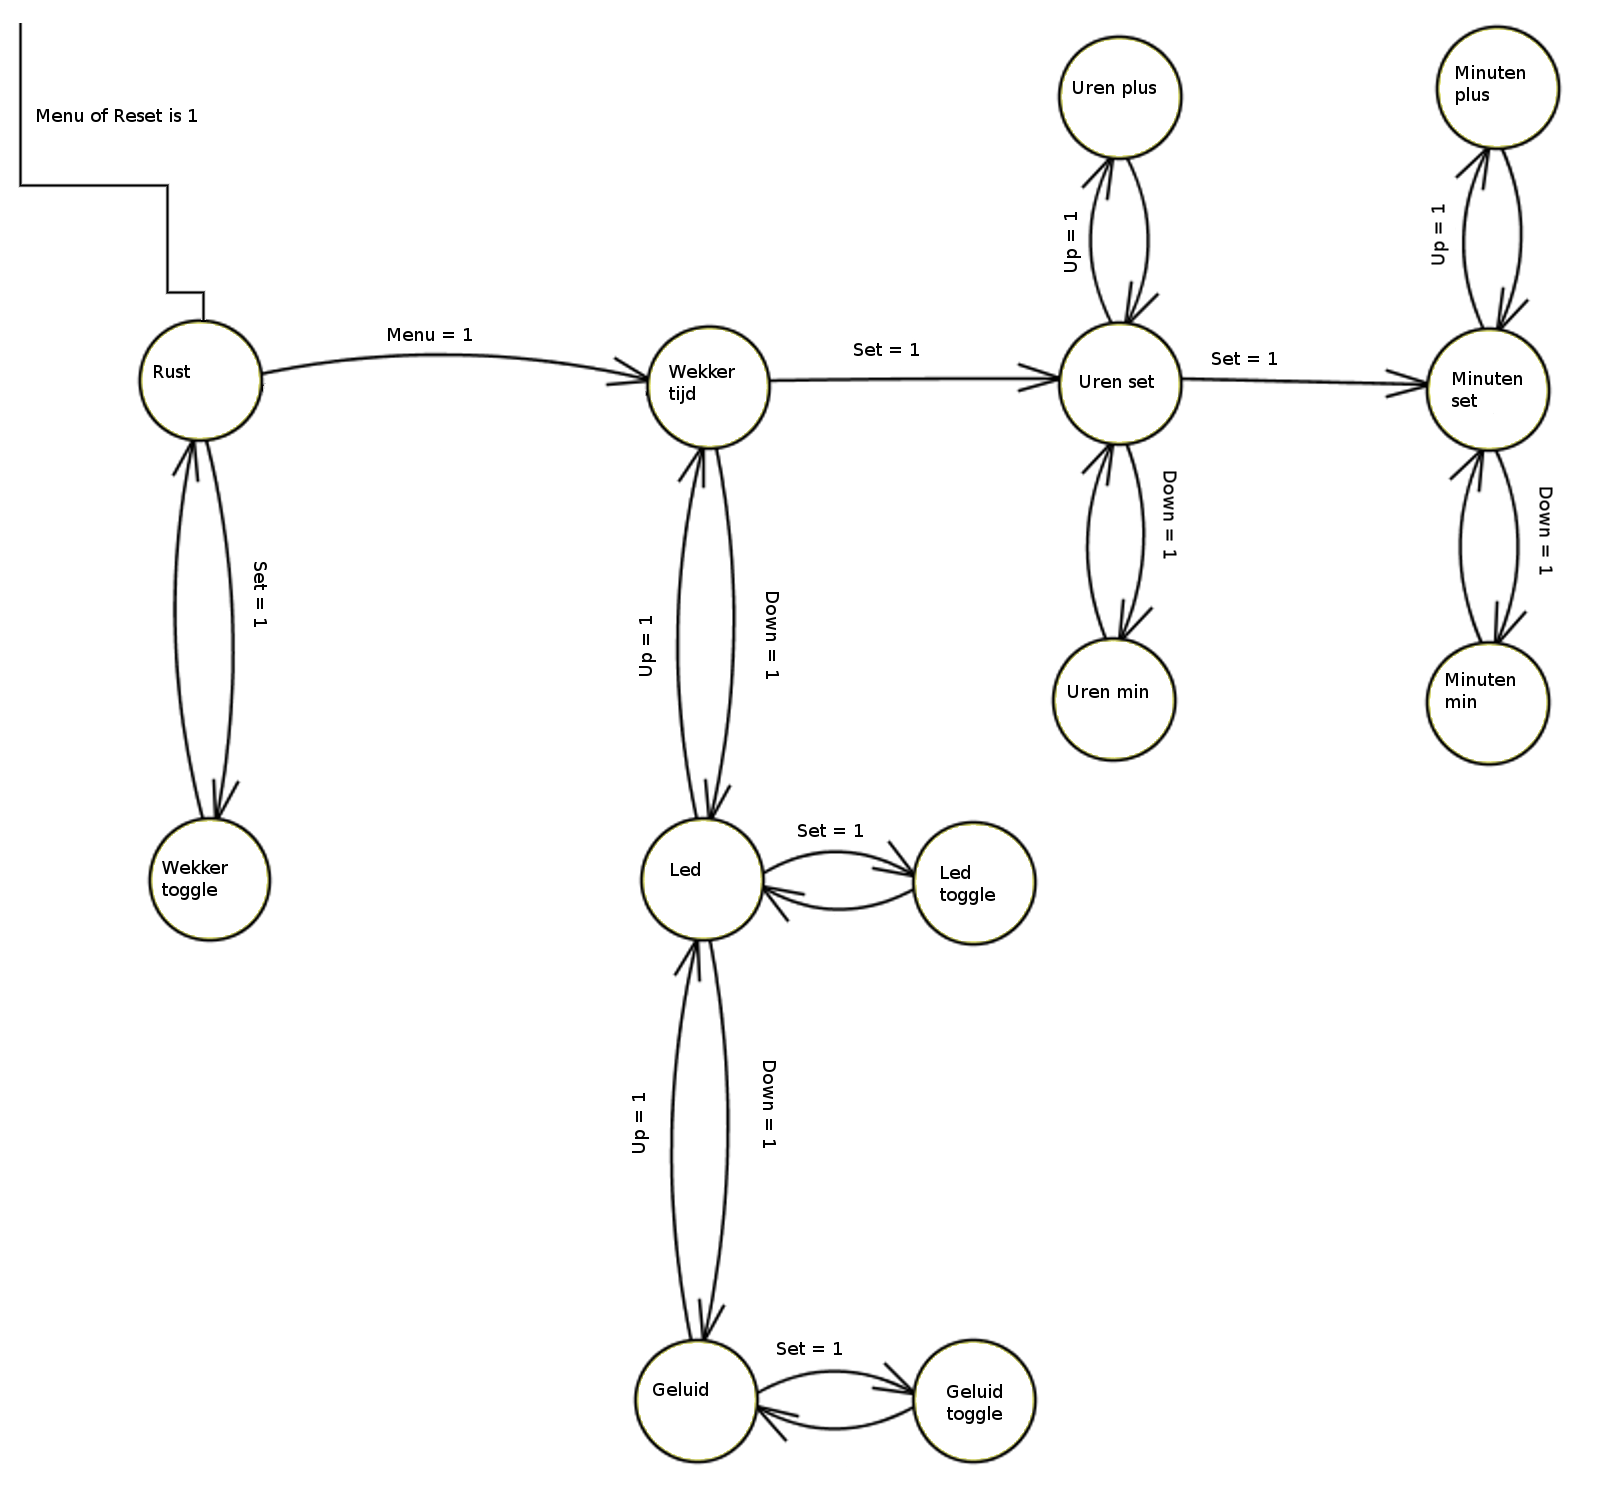
\includegraphics[width=\textwidth,height=\textheight,keepaspectratio]{Figuren/Controller/FSM_controller.png}
\caption{FSM diagramma van de menu}
\label{fig:FSM_controller}
\end{figure}

\begin{longtable}{|l| p{10cm} |}
\hline
Rust, Reset &
enable = '0' \newline
wekker=wekdata \newline
menu= "000" \\ \hline
Wekker toggle &
enable = '1' \newline
wekker[12 down to 0]=wekdata[12 down to 0] \newline
wekker[13]= niet wekdata[13] \newline
menu = "000" \\ \hline
Wekkertijd &
enable ='0' \newline
wekker=wekdata \newline
menu = "000" \\ \hline
Led &
enable ='0' \newline
wekker=wekdata \newline
menu = "011" \\ \hline
Led toggle &
enable ='1' \newline
wekker[11 down to 0]=wekdata[11 down to 0]\newline
wekker[12] = niet wekdata[12] \newline
wekker[13] = wekdata[13] \newline
menu = "011" \\ \hline
Geluid & 
enable ='0' \newline
wekker=wekdata \newline
menu = "100" \\ \hline
Geluid toggle &
enable ='1' \newline
wekker[10 down to 0]=wekdata[10 down to 0] \newline
wekker[11] = niet wekdata[11] \newline
wekker[13 downto 12] = wekdata[13 downto 12] \newline
menu = "100" \\ \hline
Tijd uren &
enable ='0' \newline
wekker=wekdata \newline
menu = "001" \\ \hline
Uren plus &
enable ='1' \newline
wekker=wekdata+1 \newline
menu = "001" \\ \hline
Uren min &
enable ='1' \newline
wekker=wekdata-1 \newline
menu = "001" \\ \hline
Tijd minuten &
enable ='0' \newline
wekker=wekdata \newline
menu = "010" \\ \hline
Minuten plus &
enable ='1' \newline
wekker=wekdata+1 \newline
menu = "010" \\ \hline
Minuten min &
enable ='1' \newline
wekker=wekdata-1 \newline
menu = "010" \\ \hline
\caption{Uitgangen binnen de state van de controller} 
\label{tab:states_controller}
\end{longtable}

\subsection{VHDL code}
De code voor de controller van de wekker is te vinden in \cref{Ap:code_controller}. Voor de overzicht en het modular opbouwen is de code in vier blokken geschreven.
\begin{itemize}[nolistsep]
\item De top entity met de port map. Deze is te vinden in \cref{code:controller_ent,code:controller_beh}.
\item Het menu, hierin zit de echte logica verwerkt. Deze is te vinden in \cref{code:menu_ent,code:menu_beh}.
\item Het gebruikte geheugen element voor de opslag van 14 bits, te vinden in \cref{code:geheugen_ent,code:geheugen_beh}.
\item De gebruikte buffer is te vinden in \cref{code:buffer_ent,code:buffer_beh}. De buffer regelt het ingangssignaal, en zorgt ervoor dat er maar 1 klokperiode lang een hoog signaal gelezen word.
\end{itemize}
Voor het testen van de code zijn er testbenches gemaakt welke te vind zijn in \cref{code:tb_controller,code:tb_menu,code:tb_geheugen,code:tb_buffer}.

\section{Testen}
Om zeker te zijn dat alles goed werkt worden er drie verschillende testen uitgevoerd. De eerste is op behavioural niveau. Hier wordt getest of de basis van de code werkt zoals verwacht. Na een goed geslaagd resultaat kan de code worden gesynthetiseerd, en deze gesynthetiseerde code worden gesimuleerd. Als er geen fouten optreden kan het ontwerp gemaakt worden, daarna geextraheerd en nogmaals getest worden. De testen worden uitgevoerd met behulp van \emph{Modelsim}.


\section{Simulatie}
De resultaten van de simulatie staan in \cref{Ap:sim_controller}. De testbench is te lang om in een keer weer te geven daarom is deze op geknipt in vier stukken. De testbench die gemaakt is voor de simulatie staat in \cref{code:tb_controller}
\section{Resultaten}
Van \cref{fig:sim_beh_0-2_5} tot en met \cref{fig:sim_ext_7_5-} is te zien dat iedere simulatie tot hetzelde resultaat leid en daarmee succesvol is.
De minimale klokperiode kan afgelezen worden aan de hand van \cref{fig:timing_controller}. Hieruit is op te makken dat deze 60ns is.
\subsection{Conclusie en discussie}
De controller werkt op alle gesimuleerde niveau's naar verwachting. 
De minimale klok periode bedraagt 60ns om gliches te voorkomen bij het optellen en aftrekken van uren en minuten. 
De controller maakt op dit moment gebruik van 9088 transitoren waarvan er voor de daadwerkelijke schakelingen slechts 2914 worden gebruikt. 
De controller maakt op dit moment nog gebruik van het binaire telsysteem (dat gebruik maakt van machten van 2), er bleek echter dat voor de lcd scherm BCD veel beter werkt. Dit moet nog worden geimplementeerd. Vlak nadat het inputbuffer gemaakt was kwam men er achter dat in plaats van een buffer ook de rising\textunderscore edge functie gebruikt had kunnen worden. 


\chapter{Alarm}
\section{Inleiding}
In de alarm module wordt een led aangestuurd, die 15 minuten voor de ingestelde tijd in de main controller begint met branden en steeds feller wordt naarmate de tijd verstrijkt. Als de huidige tijd gelijk is aan de ingestelde tijd brandt de led op z'n felst en gaat er een geluid af, totdat er een knop wordt ingedrukt.

\section{Specificaties}
\subsection{Ingangen}
\begin{itemize}[nolistsep]
\item Klok, standaard input.
\item Reset, standaard input.
\item Tijd-uur, huidige tijd in uren.
\item Tijd-minuut, huidige tijd in minuten.
\item Wekker-uur, uur ingesteld in de main controller.
\item Wekker-min, minuten ingestels in de main controller.
\item Sec, seconde signaal gegenereerd in de DCF controller.
\item Knop, alarm uitschakelen.
\end{itemize}

\subsection{Uitgangen}
\begin{itemize}[nolistsep]
\item PWM-signaal, signaal om de led aan te sturen.
\item Geluid, signaal om een geluid af te laten gaan.
\end{itemize}

\subsection{Gedrag}
Het alarm moet een bepaalde tijd voordat de wekker is ingesteld aangaan, nu gekozen voor 15 minuten.
Er wordt 15 minuten van de ingestelde tijd afgetrokken. Zodra die tijd gelijk is aan de huidige tijd komt er een signaal (licht) aan bij het gedeelte wat voor een pwm signaal zorgt.
In dat gedeelte wordt een pwm signaal gegenereerd dat elke 15 seconde breder wordt. Dit wordt gedaan door in een counter 15 seconde te tellen. Elke 15 seconde wordt de variable "lenght" kleiner. Deze begon op 64 en wordt vergeleken met een andere counter die elke klokflank telt, tot 64. Als de counter groter of gelijk is aan "length" dan is het pwm-signaal hoog. 
Als 15 minuten zijn verstreken na het aangaan van de led, dus de ingestelde tijd is gelijk aan de huidige tijd, brandt de led op z'n felst. Ook zal dan een "geluid" signaal naar '1' gaan. Dit blijft zo totdat de knop wordt ingedrukt of alles wordt gereset.
\chapter{LCD controller}
\section{LCD Controller}
Op de LCD zal de huidige tijd, ingestelde wekkertijd, datum en ingeschakelde functies te zien zijn. Een LCD is daar handig voor omdat het veel ontwerp vrijheid bied. Dat neemt ook mee dat het erg gecompliceerd kan worden. Het LCD dat zal worden gebruikt is van de fabrikant MIDAS, typenummer MC128064B6W-BNMLW~\cite{Datasheet_lcd}. Het betreft een graphical LCD van 128 x 64 pixels met een register die geschreven kan worden. De bibliotheek met characters en de controller om het LCD te schrijven zal extern van deze chip plaatsvinden door middel van een atmega32-16pu~\cite{Datasheet_micro}. Deze keuze is gemaakt omdat voor de characters niet genoeg ruimte is op de chip. De LCD controller op de chip zal dus alleen de inkomende data moeten omzetten naar een positie waarnaar het geschreven moet worden en een bijbehorend character. De layout van het display is al vastgesteld, zodat de posities alvast bekend zijn.  Zie voor de layout afbeelding \ref{fig:lcdlayout}.  \\

\begin{figure}
  \centering
     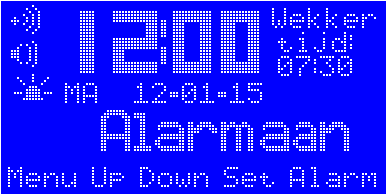
\includegraphics[angle = 0, scale= 1]{Figuren/LCD/voorbeeld_lcd.png}
       \caption{LCD layout}
\label{fig:lcdlayout}
\end{figure}

\section{Specificaties}

\begin{center}
\label{table:uitgangen}
\begin{tabular}{| l | l | p{4.5cm} |}
\hline
\textbf{Naam} & \textbf{Type} & \textbf{Functie} \\ \hline
clk           				& in std$\_$logic           									& Klok             \\ \hline
reset         			& in std$\_$logic           									& Reset            \\ \hline
ready					& in std$\_$logic 											&  \\ \hline
uren						&in std$\_$logic$\_$vector(5 downto 0) 		&data signaal met actuele uren afkomstig van DCF \\ \hline
minuten				&in std$\_$logic$\_$vector(6 downto 0) 		&data signaal met actuele minuten afkomstig van DCF \\ \hline
dagvdweek			&in std$\_$logic$\_$vector(2 downto 0)			&data signaal met de actuele dag afkomstig van DCF\\ \hline
dagvdmaand		&in std$\_$logic$\_$vector(5 downto 0) 		&data signaal met de actuele dag van de maand afkomstig van DCF \\ \hline
maand					&in std$\_$logic$\_$vector(4 downto 0) 		&data signaal met de actuele maand afkomstig van DCF  \\ \hline
jaar						&in std$\_$logic$\_$vector(7 downto 0)	 		&data signaal met het actuele jaar afkomstig van DCF  \\ \hline
dcf$\_$debug		&in std$\_$logic 												&signaal afkomstig van het dcf component en weergeeft of het DCF signaal ontvangen wordt of niet \\ \hline
menu					&in std$\_$logic$\_$vector(2 downto 0)			&data signaal die de actuele menu state weergeeft \\ \hline
alarm 					&in std$\_$logic												&buffer signaal dat weergeeft of alarmfunctie in of uitgeschakeld is\\ \hline
geluid$\_$signaal 		&in std$\_$logic 		 										&buffer signaal dat weergeeft of geluidsfunctie in of uitgeschakeld is \\ \hline
licht$\_$signaal 	&in std$\_$logic 		 										&buffer signaal dat weergeeft of lichtfunctie in of uitgeschakeld is  \\ \hline 
wektijd$\_$uren 	& in std$\_$logic$\_$vector(5 downto 0)		&data signaal met ingestelde wektijd uren \\ \hline 
wektijd$\_$min 	&in std$\_$logic$\_$vector(6 downto 0) 		&data signaal met ingestelde wektijd minuten \\ \hline 
data$\_$out 		&out std$\_$logic$\_$vector(6 downto 0) 		&data signaal dat de x,y,c informatie doorgeeft aan de microcontroller \\ \hline 
clk$\_$out 			&out std$\_$logic 		 										&clock om microcontroller clock mee te synchroniseren \\ \hline 
\end{tabular}
\end{center}

\newpage
\begin{figure}
  \centering
     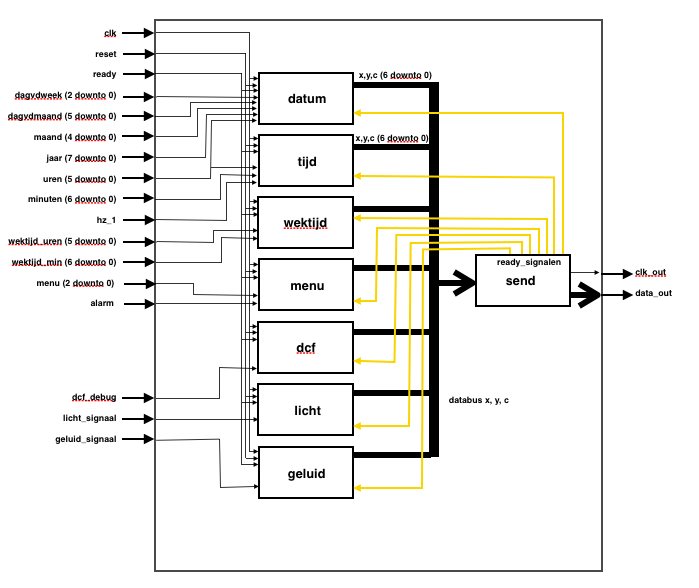
\includegraphics[angle = 0, scale= 0.5]{verslag_schemas/toplevel_entity.png}
       \caption{Toplevel Entity}
\label{fig:lcdtoplevel}
\end{figure}
\newpage

\subsection{Gedrag}
De LCD controller zal na de reset alle informatie die hij binnen krijgt omzetten naar een karakter met bij behorende x en y positie en wegschrijven naar de microprocessor van de LCD. Daarna zal de controller alleen de data die veranderd op de ingangen omzetten en  wegschrijven naar de microprocessor om tijd en onnodige acties te besparen. \\
Het verzenden van de x,y en c gaat door een data signaal van 7 bits samen met een clock$\_$out. Een neergaande klokflank geeft aan dat de data klaar staat om te verzenden zodat er op de opgaande klokflank kan worden gesampled. Zo zal eerst de x, daarna de y en als laatste de c worden verzonden. Het versturen van een karakter duurt dus 3 klokslagen van de clock$\_$out. een klokslag van de clock$\_$out is gelijk aan 2 klokslagen van de ingaande clk. 

\section{Functionaliteit}
De systemen links (datum, tijd, etc)  zorgen per stuk voor het ontvangen van de inkomende informatie en het omzetten naar een x,y positie met een karakter. De x,y en de c zal op de uitgang van het component worden gezet. 
Het component send$\_$buffer is een MUX en zorgt voor het uitlezen van de x,y en c en zal door middel van de ready signalen aangeven welk signaal hij heeft uigelezen en naar de zender heeft verstuurd. Zodra de ready laag wordt, weet het desbetreffende component dat de data is uitgelezen en zal daarna nieuwe data klaar zetten. 
Nadat de mux de data naar de zender heeft gebufferd, zal de zender de signalen een voor een door  verzenden naar de microcontroller. Tegelijkertijd zal de zender een clock$\_$out geven, zodra de clock laag wordt staat de data klaar, zodat op de opgaande klokflank de data vanaf de chip kan worden uitgelezen. 

\section{Subsystemen LCD}

\subsection{Datum}
\subsubsection{Gedrag}
Na een reset of \'e\'en keer per dag om 12 uur middernacht zal het datum component de data voor de nieuwe datum verzenden naar de zend buffer. De inkomende data is in het binary coded decimal (bcd) formaat. Eerst zal hij de dag van de week doorgeven, daarna de dag van de maand, de maand en daaropvolgend het jaartal. Dat allemaal sequentieel, getriggert op de neergaande klokflank van de ready$\_$buf. 

\begin{figure}
  \centering
     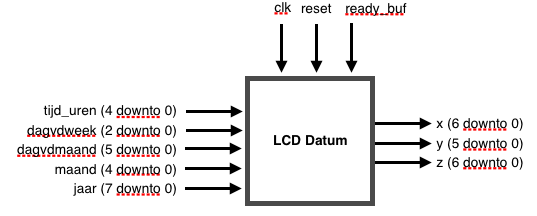
\includegraphics[angle = 0, scale= 0.75]{verslag_schemas/datum_entity.png}
       \caption{Entity datum}
\label{fig:datumentity}
\end{figure}


\subsubsection{Functionaliteit}
Het component werkt met een finite state machine (FSM) waarin de characters worden klaargezet en een counter genaamd positie wordt aangestuurd met daarnaast een apart process om de juiste input te bepalen afhankelijk van de counter. \\
Na de reset zal de FSM in de selectdata state starten en positie op 0 worden gezet. 
In het aparte process zal de de data$\_$buf worden gekoppeld aan de input die hoort bij positie=0 en zal de x en y bepaald worden. 
 In selectdata zal  afhankelijk van de counter (in dit geval 0) worden bepaald of de dag van de week of de getallen van de datum moet worden geschreven. Bij positie=0 zal het karakter van de dag van de week (in state cdvdw) worden klaargezet. Het karakter wordt bepaald door de waarde die op de data$\_$buf staat. Op de neergaande klokflank van het ready$\_$buf signaal zal de FSM terug gaan naar de state selectdata en zal er bij positie 1 worden opgeteld. Daardoor zal hierna het eerste getal van de datum worden geschreven. Dit zal zich herhalen tot positie =7, daarna zal hij naar de rust stand gaan en is de datum geschreven. \\
 Als het middernacht is, dus tijd$\_$uren = '00000', zal er ook een nieuwe datum worden klaargezet. Zodra de positie 7 is zal de machine in state selectdata blijven hangen totdat de tijd$\_$uren ongelijk is aan "00000". Dit om te voorkomen dat het component een uur lang onnodig data blijft verzenden. 


\subsubsection{FSM}
\begin{figure}
  \centering
     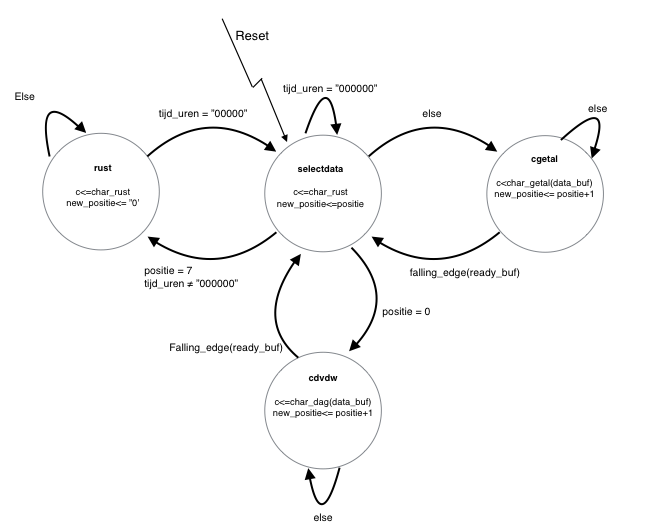
\includegraphics[width=15cm]{verslag_schemas/datum_fsm.png}
       \caption{FSM Datum}
\label{fig:lcddatumfsm}
\end{figure}

\subsubsection{VHDL code}
Zie \ref{code:ent_datum} voor de entity code. \\
Zie \ref{code:beh_datum} voor de behavioural code.\\
Zie \ref{code:tb_datum} voor de testbench die is gebruikt.
\subsubsection{Simulaties}
Zie \ref{fig:sim_datum_behavioural} voor de simulatie van de behavioural code. \\
Zie \ref{fig:sim_datum_circuit} voor de simulatie van het gesynthetiseerde circuit. 
De simulaties zijn uitgevoerd met een clock van 2000ns.  Er is getest tot 300k ns, zie de testbench in \ref{code:tb_datum} voor meer informatie.

\subsubsection{Resultaten}
Uit de simulaties is gebleken dat het circuit doet waarvoor het is ontworpen.

\subsection{Tijd en Wektijd}

\subsubsection{Gedrag}
Na een reset of bij het veranderen van de minuten zal de entity tijd data gaan verzenden. De data die verzonden wordt bevat informatie over welk character geprint moet worden en zijn positie. De characters die moeten worden verzonden worden bepaalt aan de hand van de minuten en uren die de entity in gaan. Dit zal altijd op de volgende volgorde gaan: tientallen uren, eentallen uren, tientallen minuten en als laatste eentallen minuten. Ook zal de module bij een opgaande flank van het \'e\'en Hz signaal de dubbele punt tussen de uren en minuten aan of uit zetten.\\
Het component wektijd verzend dezelfde informatie naar het LCD, alzij het op een andere positie. De wektijd zal beginnen met verzenden op het moment dat de wektijd wordt aangepast in het menu. De volgorde van de

\subsubsection{Functionaliteit}
Het component werkt volgens het Moore principe. Om de seconde wordt een nieuw character naar het LCD gestuurd. Dit character is voor de dubbele punt tussen de uren en minuten. Als er een minuut om is dan zal de nieuwe tijd naar het LCD worden verzonden.

\subsubsection{FSM}

\subsubsection{VHDL code}

\subsubsection{Simulaties}

\subsubsection{Testen}

\subsubsection{Resultaten}

\subsubsection{Discussie}

\input{LCD_controller/menu}
\input{LCD_controller/dcf}
\input{LCD_controller/geluidenlicht}
\subsection{Zender}

\subsubsection{Gedrag}
De zender zorgt ervoor dat de x, y en c van de verschillende componenten bij de microcontroller komen. Dit doet het component door een x, y en c waarde in te nemen, en deze vervolgens in de goede volgorde op de uitgang te zetten. De zender zal altijd beginnen met de x op de uitgang te zetten. Daarna zal de zender het signaal clk\_out omlaag brengen, om op de volgende klokslag dit signaal weer hoog te maken. Op de volgende klokflank zal clk\_out weer omlaag gebracht worden en y op de uitgang gezet worden. Daarna zal clk\_out weer hoog worden en zal het geheel nog herhaald worden voor de c. Nadat deze reeks is verzonden zal er bekeken worden of het volgende blok data wil verzenden. Als dit het geval is dan zal deze data verzonden worden. Mocht dat niet het geval zijn dan wordt dat blok overgeslagen en gaat de zender naar het volgende blok.

\subsubsection{Functionaliteit}
Het doel van de zender is om de data die de afzondelijke componenten willen verzenden, goed naar de microcontroller worden verzonden. Dit moet goed door de microcontroller begrepen worden. Daarom zal de volgorde van de verzonden data altijd hetzelfde zijn. Tussen twee verschillende blokken data zit altijd een beetje extra tijd. Dit is minimaal 1 klokslag. Hierdoor weet de microcontroller dat de vorige transmissie afgelopen is en dat het volgende blok weer bij de x begint.\\
Alle blokken kunnen tegelijk verzenden. De blokken moeten namelijk op een ready signaal wachten van de zender. Vervolgens selecteert de verzender via een bus naar welk blok wordt gekeken om data te verzenden. Mocht dit blok niks te verzenden hebben dan zal de c van dat blok op ''0000000'' staan. Hierdoor weet de zender dat het niks hoeft te verzenden en zal naar het volgende blok gaan.

\subsubsection{FSM}
De FSM van de zender is te vinden in \ref{fig:fsm_zender}
\begin{figure}[h!]
	\center
	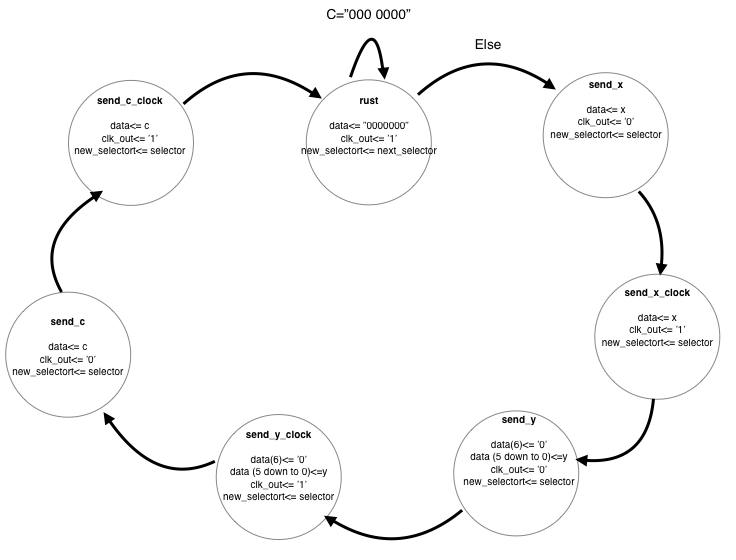
\includegraphics[width = 15cm]{Figuren/LCD/fsm_sender.png}
	\caption{FSM van component zender}
	\label{fig:fsm_zender}
\end{figure}

\subsubsection{VHDL code}
De vhdl code van de zender is opgedeeld in twee stukken, namelijk een send control en een send bus. Deze twee zijn vervolgens met een structural behaviour bij elkaar gevoegd. De code van de send control is te vinden in \ref{code:ent_send_control} en \ref{code:beh_send_control}. De code voor de send bus is te vinden in \ref{code:ent_send_bus} en \ref{code:beh_send_bus}. De top structure is te vinden in \ref{code:ent_send_top} en \ref{code:struc_send_top}.

\subsubsection{Simulaties}
De simulatie van de gehele zender is te vinden in \ref{fig:sim_send_top}. Hierin is goed te zien dat ready voor elk blok apart omhoog gaat en dat het blok voor blok behandeld wordt. Deze simulatie is gedaan met de testbench in \ref{code:tb_send_top}.

\subsubsection{Resultaten}
De simulatie is zoals te verwachten valt. Hierdoor kan geconcludeert worden dat de zender naar behoren werkt.

\subsection{VHDL code}
Zie \ref{code:ent_lcd_top} voor de entity code. \\
Zie \ref{code:beh_lcd_top} voor de behavioural code.\\
Zie \ref{code:tb_lcd_top} voor de testbench die is gebruikt.

\section{Simulatie}
Zie \ref{fig:sim_lcdtop} voor de simulatie van de behavioural code. \\

\section{Testen}
Tijdens het testen van verschillende subcircuits zijn veel dingen fout gegaan. Vaak waren de circuits dan ook wel goed, maar was de testbench niet correct. Zo hebben we in het begin met een te hoge clock frequentie getest, maar ook met signalen die niet lang genoeg hoog bleven. \\
Het systeem is ook getest op een Altera FPGA bord. Eerst dachten we dat het niet werkte, maar achteraf bleek dat, wat best logisch is,  het systeem zodanig snel werkt dat wij zelf het niet konden waarnemen. Door de klok te pulsen met een button konden we zien dat het systeem weldegelijk correct werkt.

\section{Resultaten}
De resultaten zijn goed. Het systeem heeft 2 errors in de switch level simulatie. Dat heeft te maken met de testbench waarin een situatie wordt gecre\"eerd die zich nooit zal voordoen. Dat maakt dus niks uit.

\subsection{Conclusie en discussie}
De controller werkt naar verwachting. Omdat vanwege tijdgebrek en gestelde prioriteiten de microcontroller nog niet af is voor het LCD kan nog niet worden getest of het systeem ook daarmee goed functioneerd. Al verwachten wij, omdat de simulaties en de test op de FPGA positief zijn, dat het kan gaan werken.\\


\chapter{Results for total design}
Alle subblokken moeten in een top-entity aan elkaar geknoopt worden. Deze code is te vinden in appendix \ref{code:top-level-entity}. Om dit te testen is er een simulatie gedaan. Het resultaat daarvan is te vinden in figuur \ref{fig:uiteinres}.

\begin{figure}[h!]
\includegraphics[width=\textwidth]{behaviour}
\caption{Simulatie resultaat}
\label{fig:uiteinres}
\end{figure}

Hieruit blijkt dat de chip voldoet aan de gestelde eisen. Om een beter beeld te krijgen of deze resultaten eruit komen als de chip daadwerkelijk ontwikkeld is, is er ook de gesynthetiseerde code gesimuleerd. Het resultaat daarvan is te vinden in figuur \ref{fig:uiteinsimres}.

\begin{figure}[h!]
\includegraphics[width=\textwidth]{synthesised.png}
\caption{Gesynthetiseerd resultaat}
\label{fig:uiteinsimres}
\end{figure}

Na deze te hebben vergeleken, bleken die goed overeen te komen.
\chapter{Plan voor het testen van de chip}
%Moet het gaan over het testen van de daadwerkelijke gemaakte chip in Q4 of moet het gaan over het testen op de fpga
Voor het testen zijn een aantal momenten in het proces waarop getest wordt. Zo wordt elk module getest in een simulatie in Modelsim. Hieruit kan opgemaakt worden wat het verwachte gedrag is. Maar een simulatie is niet alles. Daarom kan een module ook nog getest worden door middel van een FPGA te programmeren. De uiteindelijke chip zal getest worden met een logic analyzer en natuurlijk door te kijken of de chip de gewenste output geeft.
\section{FPGA bord}
Het bord dat gebruikt kan worden is een Altera FPGA bord. Dit bord komt met eigen software genaamt Quartus. Deze software kan gebruikt worden om de gemaakte VHDL code om te zetten in een bitstream file en vervolgens het FPGA bord te programmeren. Door de VHDL code op een FPGA te programmeren kan worden geverifieerd of de code het gedrag vertoont wat verwacht wordt. Door simulatie is dit namelijk niet altijd helemaal te zien. Mocht op de FPGA een fout ontdekt worden, dan zal de code hierop aangepast worden en zal de code opnieuw gesimuleerd worden.
\section{Logic Analyzer}
De gemaakte chip zal in Q4 worden getest. De chip zal eerst op een logic analyzer worden aangesloten. De analyzer die gebruikt zal worden is een LA-5580.

\chapter{Voortgang van het project}

\section{Inleiding}
Bij dit project zijn er vaak weinig resultaten, totdat het bijna afgelopen is. 
Dit is een van de redenen dat voor een wake-up light gekozen is.
Een wekker zelf is relatief makkelijk te maken. 
Er zijn echter ook een hele hoop extra features die in een wekker geimplementeerd kunnen worden. 
Op deze manier is dus een werkend resultaat relatief snel geproduceerd, en kunnen daarna naar gelang extra toepassingen toegevoegd worden. 
Dit is goed voor het moreel in de groep, aangezien een werkend product al heel snel gerealiseerd is.
Hierdoor is er ook meer aansporing om meer toepassingen te implementeren, omdat er al een werkend geheel is. 
In het ergste geval is er geen extra feature.
Daarnaast, als uiteindelijk bleek dat de planning te krap was, kunnen er features geschrapt worden, en is er nog steeds een werkend product. 
Onder andere dit maakt een wake-up light zeer aantrekkelijk om te maken.

\section{Werkverdeling}
Zodra duidelijk was wat gemaakt ging worden, werd een werkplan opgesteld.
Dit was nodig zodat het duidelijk was wat er gedaan moest worden.
Vervolgens zijn de taken zo snel mogelijk verdeeld door de wake-up light in blokken te verdelen. 
Van deze blokken werden ook eerst de specificaties bepaald, zodat er geen communicatieproblemen zouden ontstaan tussen de blokken.
Uiteindelijk zijn er 4 hoofdblokken ontstaan, wat goed uitkwam, aangezien dit betekende dat er weer 4 tweetallen nodig waren, en de groep bestaat uit 8 mensen. \\
Deze blokken werden vervolgens door de tweetallen apart gemaakt, en waar de specificaties niet duidelijk genoeg waren, of onhandig gedefinieerd, werden deze aawngepast. 


\section{Samenwerking binnen de groep}


\section{Afspraken binnen de groep}
Afspraken binnen de groep verliepen soepel. De enkele keer dat dit niet gebeurde was hier een goede reden voor. Zo gebeurde het dat op de dag van een presentatie bleek dat een van de leden ziek was. Andere leden sprongen in en zo kwam de presentatie toch nog tot een goed einde.
\chapter{Conclusie}

Alle onderdelen zijn in theorie nu klaar. Individueel zijn ze via \emph{Modelsim} getest en goed bevonden. De onderlinge signalen zijn zo veel mogelijk op elkaar afgestemd. De onderdelen voldoen samen aan de specificaties die eerder gesteld zijn. Echter in de praktijk zullen de onderdelen nog niet feilloos met elkaar samenwerken. Hiervoor zal er meer meer getest worden, bijvoorbeeld op een FPGA bord en een logic analyzer.
% alle onderdelen voldoen aan de gestelde eisen
	% wekker wordt gesynchroniseerd
	% menu is te navigeren met 4 knoppen
	% LCD wordt goed aangestuurd  en geluid en licht doet het.
% past op de chip?
% test op modelsim?
% test op fpga?
% test switch-level?
% komt overheen
% 
% verder onderzoek:
% chip uitproberen

\appendix								% To use letters as chapter numbers (appendices)
\chapter[FSM diagrammen (DCF77)]{FSM diagrammen (DCF77 blok)}
\label{Ap: dcf_fsm}

\section*{Subblokken van synctime}
\begin{figure}[h!]
\begin{center}
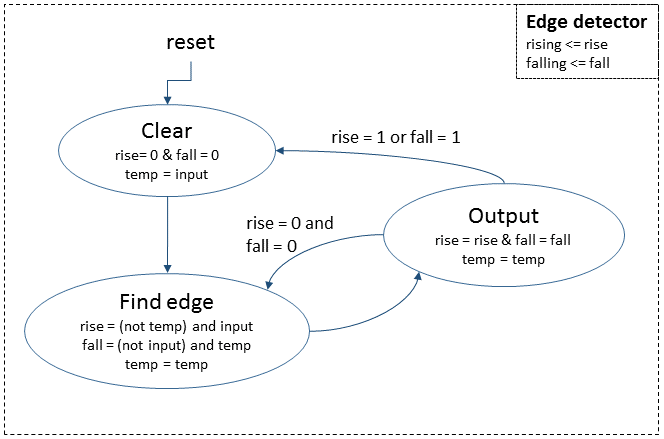
\includegraphics[keepaspectratio=true,scale=0.7]{Figuren/DCF77/FSM_edge_detector}
\captionsetup{justification=centering}\caption{FSM diagram van het subblok edge detector}
\label{fig: edge_detector}
\end{center}
\end{figure}

\begin{figure}[h!]
\begin{center}
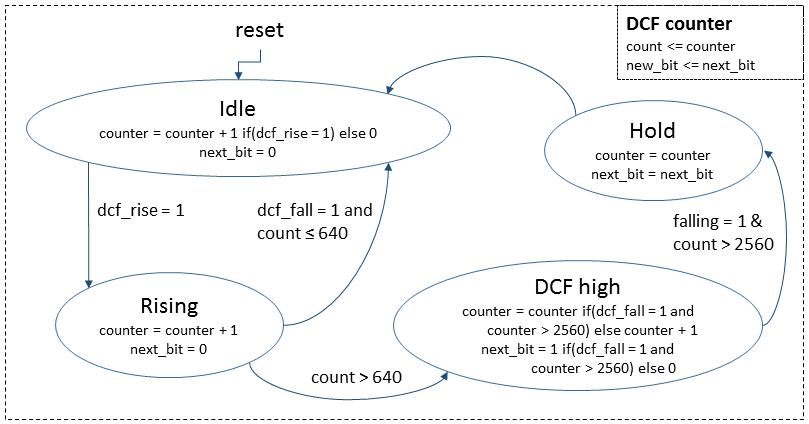
\includegraphics[keepaspectratio=true,scale=0.6]{Figuren/DCF77/FSM_counter}
\captionsetup{justification=centering}\caption{FSM diagram van het subblok DCF counter}
\label{fig: dcf_counter}
\end{center}
\end{figure}

\begin{figure}[h!]
\begin{center}
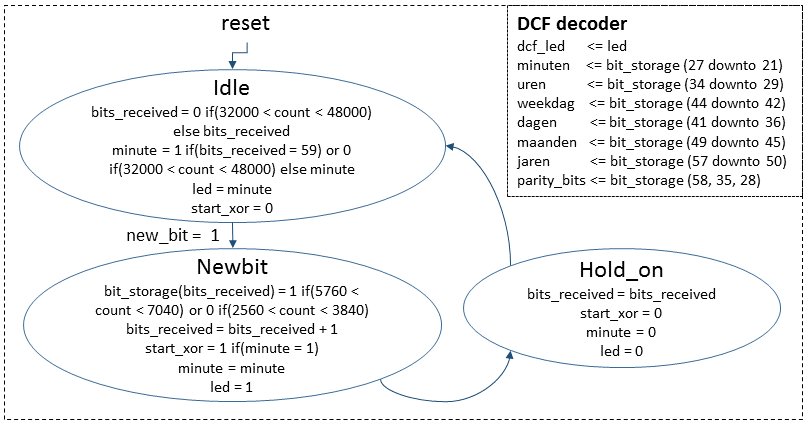
\includegraphics[keepaspectratio=true,scale=0.6]{Figuren/DCF77/FSM_decoder}
\captionsetup{justification=centering}\caption{FSM diagram van het subblok DCF decoder}
\label{fig: dcf_decoder}
\end{center}
\end{figure}

\begin{figure}[h!]
\begin{center}
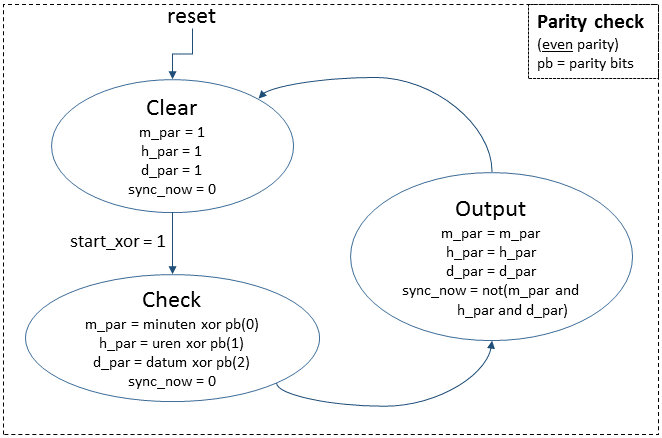
\includegraphics[keepaspectratio=true,scale=0.7]{Figuren/DCF77/FSM_parity_check}
\captionsetup{justification=centering}\caption{FSM diagram van het subblok parity check}
\label{fig: parity_check}
\end{center}
\end{figure}

\section*{Klokdeler}
\begin{figure}[h!]
\begin{center}
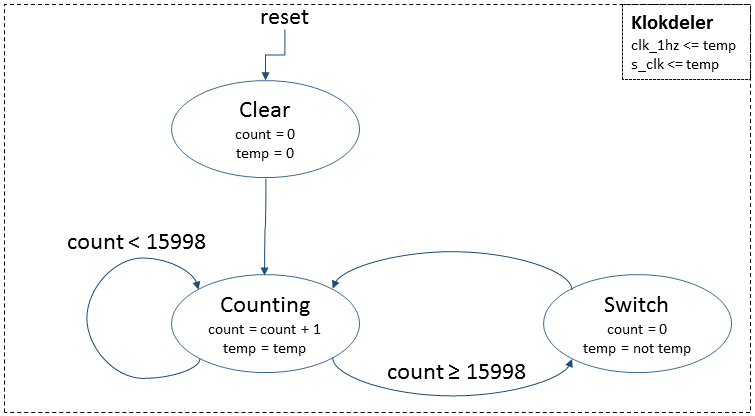
\includegraphics[keepaspectratio=true,scale=0.65]{Figuren/DCF77/FSM_klokdeler}
\captionsetup{justification=centering}\caption{FSM diagram van het subblok klokdeler}
\label{fig: klokdeler}
\end{center}
\end{figure}

\section*{Subblokken van de klok}
\begin{figure}[h!]
\begin{center}
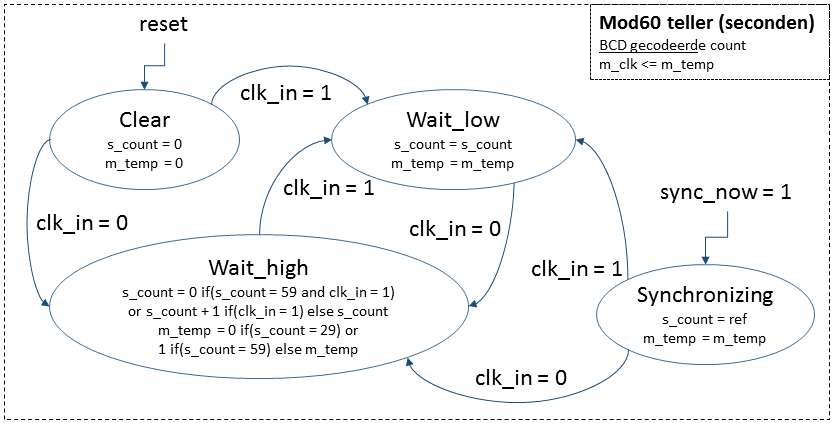
\includegraphics[keepaspectratio=true,scale=0.6]{Figuren/DCF77/FSM_seconden}
\captionsetup{justification=centering}\caption{FSM diagram van het subblok seconden teller}
\label{fig: seconden_teller}
\end{center}
\end{figure}

\begin{figure}[h!]
\begin{center}
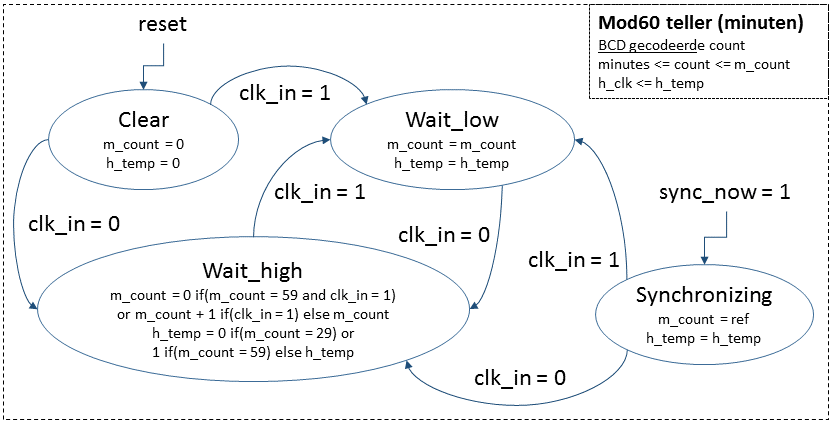
\includegraphics[keepaspectratio=true,scale=0.6]{Figuren/DCF77/FSM_minuten}
\captionsetup{justification=centering}\caption{FSM diagram van het subblok minuten teller}
\label{fig: minuten_teller}
\end{center}
\end{figure}

\begin{figure}[h!]
\begin{center}
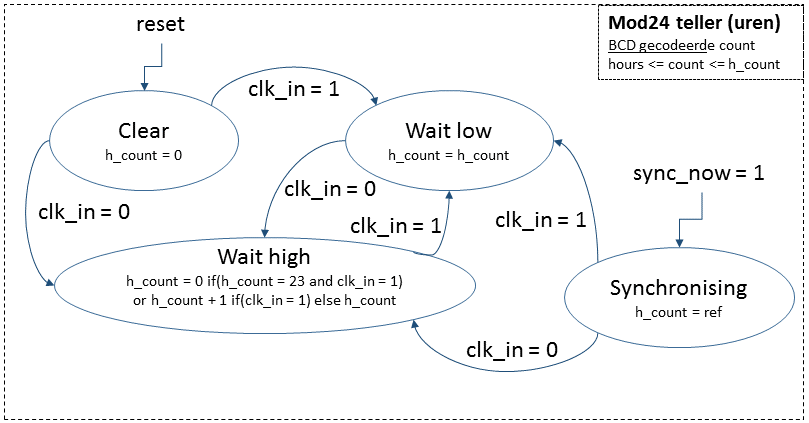
\includegraphics[keepaspectratio=true,scale=0.6]{Figuren/DCF77/FSM_uren}
\captionsetup{justification=centering}\caption{FSM diagram van het subblok uren teller}
\label{fig: uren_teller}
\end{center}
\end{figure}
\chapter[VHDL code]{Vhdl code}
\section{VHDL beschrijving van het DCF77 blok}
\label{Ap: DCF_code}
\phantomsection\subsection*{\refstepcounter{subsection}\label{code: edge_detector}\thesubsection.\quad Edge detector}
\scriptsize 
\lstinputlisting [style= VHDL]{VHDL/DCF77/edge_detector.vhd}
\hrule
\lstinputlisting [style= VHDL]{VHDL/DCF77/edge_detector-behaviour.vhd}
\normalsize
\newpage

\phantomsection\subsection*{\refstepcounter{subsection}\label{code: dcf_counter}\thesubsection.\quad DCF counter}
\scriptsize 
\lstinputlisting [style= VHDL]{VHDL/DCF77/dcf_counter.vhd}
\hrule
\lstinputlisting [style= VHDL]{VHDL/DCF77/dcf_counter-behaviour.vhd}
\normalsize

\phantomsection\subsection*{\refstepcounter{subsection}\label{code: dcf_decoder}\thesubsection.\quad DCF decoder}
\scriptsize 
\lstinputlisting [style= VHDL]{VHDL/DCF77/dcf_decoder.vhd}
\hrule
\lstinputlisting [style= VHDL]{VHDL/DCF77/dcf_decoder-behaviour.vhd}
\normalsize

\phantomsection\subsection*{\refstepcounter{subsection}\label{code: parity_check}\thesubsection.\quad Parity check}
\scriptsize 
\lstinputlisting [style= VHDL]{VHDL/DCF77/parity_check.vhd}
\hrule
\lstinputlisting [style= VHDL]{VHDL/DCF77/parity_check-behaviour.vhd}
\normalsize

\phantomsection\subsection*{\refstepcounter{subsection}\label{code: synctime}\thesubsection.\quad Synctime}
\scriptsize 
\lstinputlisting [style= VHDL]{VHDL/DCF77/synctime.vhd}
\hrule
\lstinputlisting [style= VHDL]{VHDL/DCF77/synctime-structure.vhd}
\normalsize

\phantomsection\subsection*{\refstepcounter{subsection}\label{code: klokdeler}\thesubsection.\quad Klokdeler}
\scriptsize 
\lstinputlisting [style= VHDL]{VHDL/DCF77/klokdeler.vhd}
\hrule
\lstinputlisting [style= VHDL]{VHDL/DCF77/klokdeler-behaviour.vhd}
\normalsize

\phantomsection\subsection*{\refstepcounter{subsection}\label{code: mod60_clk}\thesubsection.\quad Mod60 (seconden) teller}
\scriptsize 
\lstinputlisting [style= VHDL]{VHDL/DCF77/mod60_clk_bcd.vhd}
\hrule
\lstinputlisting [style= VHDL]{VHDL/DCF77/mod60_clk_bcd-behaviour.vhd}
\normalsize

\phantomsection\subsection*{\refstepcounter{subsection}\label{code: mod60_tel}\thesubsection.\quad Mod60 (minuten) teller}
\scriptsize 
\lstinputlisting [style= VHDL]{VHDL/DCF77/mod60_tel_bcd.vhd}
\hrule
\lstinputlisting [style= VHDL]{VHDL/DCF77/mod60_tel_bcd-behaviour.vhd}
\normalsize

\phantomsection\subsection*{\refstepcounter{subsection}\label{code: mod24_tel}\thesubsection.\quad Mod24 (uren) teller}
\scriptsize 
\lstinputlisting [style= VHDL]{VHDL/DCF77/mod24_tel_bcd.vhd}
\hrule
\lstinputlisting [style= VHDL]{VHDL/DCF77/mod24_tel_bcd-behaviour.vhd}
\normalsize

\phantomsection\subsection*{\refstepcounter{subsection}\label{code: ausy_klok}\thesubsection.\quad Autonome synchroniseerbare klok}
\scriptsize 
\lstinputlisting [style= VHDL]{VHDL/DCF77/ausy_klok_bcd.vhd}
\hrule 
\lstinputlisting [style= VHDL]{VHDL/DCF77/ausy_klok_bcd-structure.vhd}
\normalsize

\phantomsection\subsection*{\refstepcounter{subsection}\label{code: dcf77}\thesubsection.\quad DCF77 (top-level)}
\scriptsize 
\lstinputlisting [style= VHDL]{VHDL/DCF77/dcf77_bcd.vhd}
\hrule
\lstinputlisting [style= VHDL]{VHDL/DCF77/dcf77_bcd-structure.vhd}
\normalsize
\newpage


\section{Testbenches voor het DCF77 blok}
\label{Ap: DCF_test}
\phantomsection\subsection*{\refstepcounter{subsection}\label{code: edge_detector_tb}\thesubsection.\quad Testbench edge detector}
\scriptsize 
\lstinputlisting [style= VHDL]{VHDL/DCF77/edge_detector_tb.vhdl}
\hrule
\lstinputlisting [style= VHDL]{VHDL/DCF77/edge_detector_tb-behaviour.vhd}
\normalsize

\phantomsection\subsection*{\refstepcounter{subsection}\label{code: dcf_counter_tb}\thesubsection.\quad Testbench DCF counter}
\scriptsize 
\lstinputlisting [style= VHDL]{VHDL/DCF77/dcf_counter_tb.vhdl}
\hrule
\lstinputlisting [style= VHDL]{VHDL/DCF77/dcf_counter_tb-behaviour.vhd}
\normalsize

\phantomsection\subsection*{\refstepcounter{subsection}\label{code: dcf_decoder_tb}\thesubsection.\quad Testbench DCF decoder}
\scriptsize 
\lstinputlisting [style= VHDL]{VHDL/DCF77/dcf_decoder_tb.vhdl}
\hrule
\lstinputlisting [style= VHDL]{VHDL/DCF77/dcf_decoder_tb-behaviour.vhd}
\normalsize

\phantomsection\subsection*{\refstepcounter{subsection}\label{code: parity_check_tb}\thesubsection.\quad Testbench parity check}
\scriptsize 
\lstinputlisting [style= VHDL]{VHDL/DCF77/parity_check_tb.vhdl}
\hrule
\lstinputlisting [style= VHDL]{VHDL/DCF77/parity_check_tb-behaviour.vhdl}
\normalsize

\phantomsection\subsection*{\refstepcounter{subsection}\label{code: synctime_tb}\thesubsection.\quad Testbench synctime}
\scriptsize 
\lstinputlisting [style= VHDL]{VHDL/DCF77/synctime_tb.vhdl}
\hrule
\lstinputlisting [style= VHDL]{VHDL/DCF77/synctime_tb-behaviour.vhd}
\normalsize

\phantomsection\subsection*{\refstepcounter{subsection}\label{code: klokdeler_tb}\thesubsection.\quad Testbench klokdeler}
\scriptsize 
\lstinputlisting [style= VHDL]{VHDL/DCF77/klokdeler_tb.vhdl}
\hrule
\lstinputlisting [style= VHDL]{VHDL/DCF77/klokdeler_tb-behaviour.vhd}
\normalsize

\phantomsection\subsection*{\refstepcounter{subsection}\label{code: mod60_clk_tb}\thesubsection.\quad Testbench mod60 (seconden) teller}
\scriptsize 
\lstinputlisting [style= VHDL]{VHDL/DCF77/mod60_clk_tb.vhdl}
\hrule
\lstinputlisting [style= VHDL]{VHDL/DCF77/mod60_clk_tb-behaviour.vhd}
\normalsize

\phantomsection\subsection*{\refstepcounter{subsection}\label{code: mod60_tel_tb}\thesubsection.\quad Testbench mod60 (minuten) teller}
\scriptsize 
\lstinputlisting [style= VHDL]{VHDL/DCF77/mod60_tel_tb.vhdl}
\hrule
\lstinputlisting [style= VHDL]{VHDL/DCF77/mod60_tel_tb-behaviour.vhd}
\normalsize

\phantomsection\subsection*{\refstepcounter{subsection}\label{code: mod24_tel_tb}\thesubsection.\quad Testbench mod24 (uren) teller}
\scriptsize 
\lstinputlisting [style= VHDL]{VHDL/DCF77/mod24_tel_tb.vhdl}
\hrule
\lstinputlisting [style= VHDL]{VHDL/DCF77/mod24_tel_tb-behaviour.vhd}
\normalsize

\phantomsection\subsection*{\refstepcounter{subsection}\label{code: ausy_klok_tb}\thesubsection.\quad Testbench autonome synchroniseerbare klok}
\scriptsize 
\lstinputlisting [style= VHDL]{VHDL/DCF77/ausy_klok_tb.vhdl}
\hrule 
\lstinputlisting [style= VHDL]{VHDL/DCF77/ausy_klok_tb-behaviour.vhd}
\normalsize

\phantomsection\subsection*{\refstepcounter{subsection}\label{code: dcf77_tb}\thesubsection.\quad Testbench DCF77 (top-level)}
\scriptsize 
\lstinputlisting [style= VHDL]{VHDL/DCF77/dcf77_tb.vhdl}
\hrule
\lstinputlisting [style= VHDL]{VHDL/DCF77/dcf77_tb-behaviour.vhd}
\normalsize
\newpage


\section{FPGA hulpbestanden van het DCF77 blok}
\label{Ap: FPGA_dcftest}
\phantomsection\subsection*{\refstepcounter{subsection}\label{code: fpga_buff}\thesubsection.\quad Date ready buffer}
\scriptsize 
\lstinputlisting [style= VHDL]{VHDL/DCF77/buff.vhd}
\normalsize

\phantomsection\subsection*{\refstepcounter{subsection}\label{code: fpga_gen32khz}\thesubsection.\quad Klokdeler 50 MHz naar 32 kHz}
\scriptsize 
\lstinputlisting [style= VHDL]{VHDL/DCF77/gen32khz.vhd}
\normalsize

\phantomsection\subsection*{\refstepcounter{subsection}\label{code: fpga_gen10hz}\thesubsection.\quad Klokdeler 50 MHz naar 10 Hz}
\scriptsize 
\lstinputlisting [style= VHDL]{VHDL/DCF77/gen10hz.vhd}
\normalsize

\phantomsection\subsection*{\refstepcounter{subsection}\label{code: fpga_dcfgen}\thesubsection.\quad DCF generator}
\scriptsize 
\lstinputlisting [style= VHDL]{VHDL/DCF77/dcf_gen.vhd}
\normalsize

\phantomsection\subsection*{\refstepcounter{subsection}\label{code: fpga_dcfswitch}\thesubsection.\quad Schakelaar voor de DCF generator}
\scriptsize 
\lstinputlisting [style= VHDL]{VHDL/DCF77/dcf_switch.vhd}
\normalsize

\phantomsection\subsection*{\refstepcounter{subsection}\label{code: fpga_switch}\thesubsection.\quad Schakelmogelijkheid tussen dag, maand en jaar}
\scriptsize 
\lstinputlisting [style= VHDL]{VHDL/DCF77/switch.vhd}
\normalsize

\phantomsection\subsection*{\refstepcounter{subsection}\label{code: fpga_sevenseg}\thesubsection.\quad Aansturing seven-segment display}
\scriptsize 
\lstinputlisting [style= VHDL]{VHDL/DCF77/sevenseg.vhd}
\normalsize
\newpage


\section{VHDL code controller}
\label{Ap:code_controller}
\subsection{Top level entity}
\scriptsize 
\lstinputlisting [style= VHDL]{VHDL/Controller/controller-entity.vhd}
\normalsize
\label{code:controller_ent}
\subsection{Behavioural VHDL code controller}
\scriptsize 
\lstinputlisting [style= VHDL]{VHDL/Controller/controller-behaviour.vhd}
\normalsize
\label{code:controller_beh}
\subsection{Menu entity}
\scriptsize 
\lstinputlisting [style= VHDL]{VHDL/Controller/menu-entity.vhd}
\normalsize
\label{code:menu_ent}
\subsection{Behavioural VHDL code menu}
\scriptsize 
\lstinputlisting [style= VHDL]{VHDL/Controller/menu-behaviour.vhd}
\normalsize
\label{code:menu_beh}
\subsection{Memory}
\scriptsize 
\lstinputlisting [style= VHDL]{VHDL/Controller/geheugen-entity.vhd}
\normalsize
\label{code:geheugen_ent}
\subsection{Behavioural VHDL memory}
\scriptsize 
\lstinputlisting [style= VHDL]{VHDL/Controller/geheugen-behaviour.vhd}
\normalsize
\label{code:geheugen_beh}
\subsection{Entity buffer}
\scriptsize 
\lstinputlisting [style= VHDL]{VHDL/Controller/buffer-entity.vhd}
\normalsize
\label{code:buffer_ent}
\subsection{Behavioural VHDL buffer}
\scriptsize 
\lstinputlisting [style= VHDL]{VHDL/Controller/buffer-behaviour.vhd}
\normalsize
\label{code:buffer_beh}
\section{Testbenchs voor de controller}
\subsection{VHDL controller}
\scriptsize 
\lstinputlisting [style= VHDL]{VHDL/Controller/controller-tb-behaviour.vhd}
\normalsize
\label{code:tb_controller}
\subsection{Testbench VHDL menu}
\scriptsize 
\lstinputlisting [style= VHDL]{VHDL/Controller/menu-tb-behaviour.vhd}
\normalsize
\label{code:tb_menu}
\subsection{Testbench VHDL geheugen}
\scriptsize 
\lstinputlisting [style= VHDL]{VHDL/Controller/geheugen-tb-behaviour.vhd}
\normalsize
\label{code:tb_geheugen}
\subsection{Testbench VHDL buffer}
\scriptsize 
\lstinputlisting [style= VHDL]{VHDL/Controller/buff-tb-behaviour.vhd}
\normalsize
\label{code:tb_buffer}

\section{Vhdl code van het alarm}
\label{Ap:code_alarm}
\subsection{Entity alarm-compare}
\scriptsize 
\lstinputlisting [style= VHDL]{VHDL/Alarm/compare.vhd}
\normalsize
\label{code:ent_alarm_compare}
\subsection{Behavioural alarm-compare}
\scriptsize 
\lstinputlisting [style= VHDL]{VHDL/Alarm/compare-behaviour.vhd}
\normalsize
\label{code:beh_alarm_compare}
\subsection{Top entity alarm}
\scriptsize 
\lstinputlisting [style= VHDL]{VHDL/Alarm/alarm.vhd}
\normalsize
\label{code:ent_alarm}
\subsection{Behavioural alarm}
\scriptsize 
\lstinputlisting [style= VHDL]{VHDL/Alarm/alarm-behaviour.vhd}
\normalsize
\label{code:beh_alarm}
\subsection{Entity alarm-counter}
\scriptsize 
\lstinputlisting [style= VHDL]{VHDL/Alarm/counter.vhd}
\normalsize
\label{code:ent_alarm_counter}
\subsection{Behavioural alarm-counter}
\scriptsize 
\lstinputlisting [style= VHDL]{VHDL/Alarm/counter-behaviour.vhd}
\normalsize
\label{code:beh_alarm_counter}
\subsection{Entity alarm-pwm}
\scriptsize 
\lstinputlisting [style= VHDL]{VHDL/Alarm/pwm.vhd}
\normalsize
\label{code:ent_alarm_pwm}
\subsection{Behavioural alarm-pwm}
\scriptsize 
\lstinputlisting [style= VHDL]{VHDL/Alarm/pwm-behaviour.vhd}
\normalsize
\label{code:beh_alarm_pwm}

\section{VHDL code LCD aansturing}

\label{code:ent_lcd_top}
\subsection{Top Entity LCD}
\scriptsize 
\lstinputlisting [style= VHDL]{VHDL/LCD/lcd_top.vhd}
\normalsize
\subsection{Top Entity LCD structure}
\label{code:beh_lcd_top}
\scriptsize 
\lstinputlisting [style= VHDL]{VHDL/LCD/lcd_top-structure.vhd}
\normalsize
\subsection{Entity Tijd}
\label{code:ent_tijd}
\scriptsize 
\lstinputlisting [style= VHDL]{VHDL/LCD/tijd.vhd}
\normalsize
\label{code:beh_tijd}
\subsection{Behavioural Tijd}
\scriptsize 
\lstinputlisting [style= VHDL]{VHDL/LCD/tijd-behaviour.vhd}
\normalsize
\label{code:ent_datum}
\subsection{Entity Datum}
\scriptsize 
\lstinputlisting [style= VHDL]{VHDL/LCD/datum.vhd}
\normalsize
\label{code:beh_datum}
\subsection{Behavioural Datum}
\scriptsize 
\lstinputlisting [style= VHDL]{VHDL/LCD/datum-behaviour.vhd}
\normalsize
\label{code:ent_dcf-lcd}
\subsection{Entity DCF LCD}
\scriptsize 
\lstinputlisting [style= VHDL]{VHDL/LCD/dcf_lcd.vhd}
\normalsize
\label{code:beh_dcf-lcd}
\subsection{Behavioural DCF LCD}
\scriptsize 
\lstinputlisting [style= VHDL]{VHDL/LCD/dcf_lcd-behaviour.vhd}
\normalsize
\label{code:ent_geluid}
\subsection{Entity Geluid}
\scriptsize 
\lstinputlisting [style= VHDL]{VHDL/LCD/geluid.vhd}
\normalsize
\label{code:beh_geluid}
\subsection{Behavioural Geluid}
\scriptsize 
\lstinputlisting [style= VHDL]{VHDL/LCD/geluid-behaviour.vhd}
\normalsize
\label{code:ent_licht}
\subsection{Entity Licht}
\scriptsize 
\lstinputlisting [style= VHDL]{VHDL/LCD/licht.vhd}
\normalsize
\label{code:beh_licht}
\subsection{Behavioural Licht}
\scriptsize 
\lstinputlisting [style= VHDL]{VHDL/LCD/licht-behaviour.vhd}
\normalsize
\label{code:ent_menu_scherm}
\subsection{Entity Menu scherm}
\scriptsize 
\lstinputlisting [style= VHDL]{VHDL/LCD/menu_scherm.vhd}
\normalsize
\label{code:beh_menu_scherm}
\subsection{Behavioural menu scherm}
\scriptsize 
\lstinputlisting [style= VHDL]{VHDL/LCD/menu_scherm-behaviour.vhd}
\normalsize
\label{code:ent_wektijd}
\subsection{Entity Wektijd}
\scriptsize 
\lstinputlisting [style= VHDL]{VHDL/LCD/wektijd.vhd}
\normalsize
\label{code:beh_wektijd}
\subsection{Behavioural Wektijd}
\scriptsize 
\lstinputlisting [style= VHDL]{VHDL/LCD/wektijd-behaviour.vhd}
\normalsize
\label{code:ent_send_control}
\subsection{Entity send control}
\scriptsize 
\lstinputlisting [style= VHDL]{VHDL/LCD/send_control.vhd}
\normalsize
\label{code:beh_send_control}
\subsection{Behavioural send control}
\scriptsize 
\lstinputlisting [style= VHDL]{VHDL/LCD/send_control-behaviour.vhd}
\normalsize
\label{code:ent_send_bus}
\subsection{Entity send bus}
\scriptsize 
\lstinputlisting [style= VHDL]{VHDL/LCD/send_bus.vhd}
\normalsize
\label{code:beh_send_bus}
\subsection{Behavioural send bus}
\scriptsize 
\lstinputlisting [style= VHDL]{VHDL/LCD/send_bus-behaviour.vhd}
\normalsize
\label{code:ent_send_top}
\subsection{Entity send top}
\scriptsize 
\lstinputlisting [style= VHDL]{VHDL/LCD/send_top_entity.vhd}
\normalsize
\label{code:struc_send_top}

\section{Testbenchs voor de LCD}
\subsection{Testbench VHDL Datum}
\scriptsize 
\lstinputlisting [style= VHDL]{VHDL/LCD/TB/datum_tb-behaviour.vhd}
\normalsize
\label{code:tb_datum}
\subsection{Testbench VHDL DCF77 LCD}
\scriptsize 
\lstinputlisting [style= VHDL]{VHDL/LCD/TB/dcf_lcd_tb-behaviour.vhd}
\normalsize
\label{code:tb_dcf_lcd}
\subsection{Testbench VHDL Geluid}
\scriptsize 
\lstinputlisting [style= VHDL]{VHDL/LCD/TB/geluid_tb-behaviour.vhd}
\normalsize
\label{code:tb_geluid}
\subsection{Testbench VHDL LCD Top}
\scriptsize 
\lstinputlisting [style= VHDL]{VHDL/LCD/TB/lcd_top_tb-behaviour.vhd}
\normalsize
\label{code:tb_lcd_top}
\subsection{Testbench VHDL Licht}
\scriptsize 
\lstinputlisting [style= VHDL]{VHDL/LCD/TB/licht_tb-behaviour.vhd}
\normalsize
\label{code:tb_licht}
\subsection{Testbench VHDL Menu Scherm}
\scriptsize 
\lstinputlisting [style= VHDL]{VHDL/LCD/TB/menu_scherm_tb-behaviour.vhd}
\normalsize
\label{code:tb_menu_scherm}
\subsection{Testbench VHDL Send Bus}
\scriptsize 
\lstinputlisting [style= VHDL]{VHDL/LCD/TB/send_bus_tb-behaviour.vhd}
\normalsize
\label{code:tb_send_bus}
\subsection{Testbench VHDL Send Control}
\scriptsize 
\lstinputlisting [style= VHDL]{VHDL/LCD/TB/send_cntrl_tb-behaviour.vhd}
\normalsize
\label{code:tb_send_cntrl}
\subsection{Testbench VHDL Tijd}
\scriptsize 
\lstinputlisting [style= VHDL]{VHDL/LCD/TB/tijd_tb-behaviour.vhd}
\normalsize
\label{code:tb_tijd}
\subsection{Testbench VHDL Wektijd}
\scriptsize 
\lstinputlisting [style= VHDL]{VHDL/LCD/TB/wektijd_tb-behaviour.vhd}
\normalsize
\label{code:tb_wektijd}

\subsection{Structural send top}
\scriptsize 
\lstinputlisting [style= VHDL]{VHDL/LCD/send_top_struc.vhd}
\normalsize
\label{code:tb_send_top}


\subsection{Top-level entity}
\scriptsize 
\lstinputlisting [style= VHDL]{VHDL/top_ent_str_dcf_4.vhd}
\label{code:top-level-entity}
\normalsize
\chapter[Simulatie resultaten DCF]{Simulatieresultaten van het DCF77 blok}
\label{Ap: dcf_sim}
\phantomsection\subsection*{\refstepcounter{subsection}\label{fig: edge_beh}\thesubsection.\quad Behaviour edge detector}
\begin{figure}[ht!]
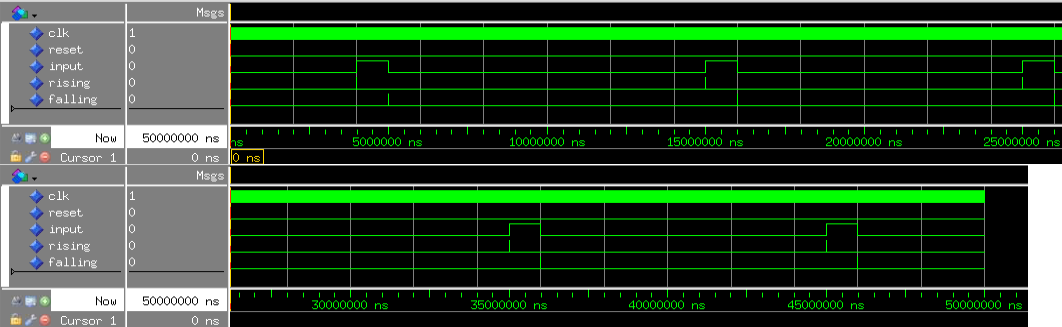
\includegraphics[width=\textwidth,height=\textheight,keepaspectratio]{Figuren/DCF77/Edge_detector.png}
\caption{Simulatie van de edge detector (50 ms op schaal)}
\end{figure}
\phantomsection\subsection*{\refstepcounter{subsection}\label{fig: count_beh}\thesubsection.\quad Behaviour DCF counter}
\begin{figure}[ht!]
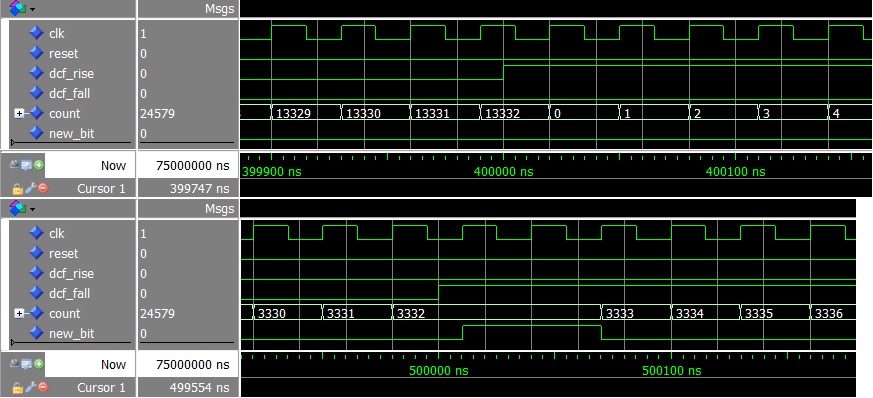
\includegraphics[width=\textwidth,height=\textheight,keepaspectratio]{Figuren/DCF77/Counter.png}
\caption{Simulatie van de DCF counter (details van 75 ms op schaal)}
\end{figure}
\phantomsection\subsection*{\refstepcounter{subsection}\label{fig: decoder_beh}\thesubsection.\quad Behaviour DCF decoder}
\begin{figure}[ht!]
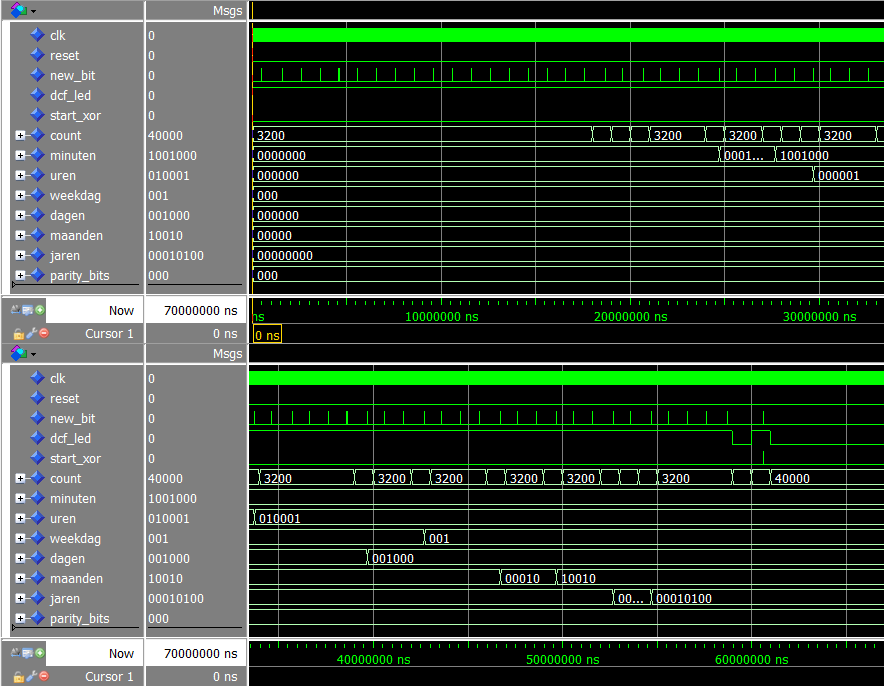
\includegraphics[width=\textwidth,height=\textheight,keepaspectratio]{Figuren/DCF77/Decoder.png}
\caption{Simulatie van de DCF decoder (70 ms op schaal)}
\end{figure}
\phantomsection\subsection*{\refstepcounter{subsection}\label{fig: parity_beh}\thesubsection.\quad Behaviour parity check}
\begin{figure}[ht!]
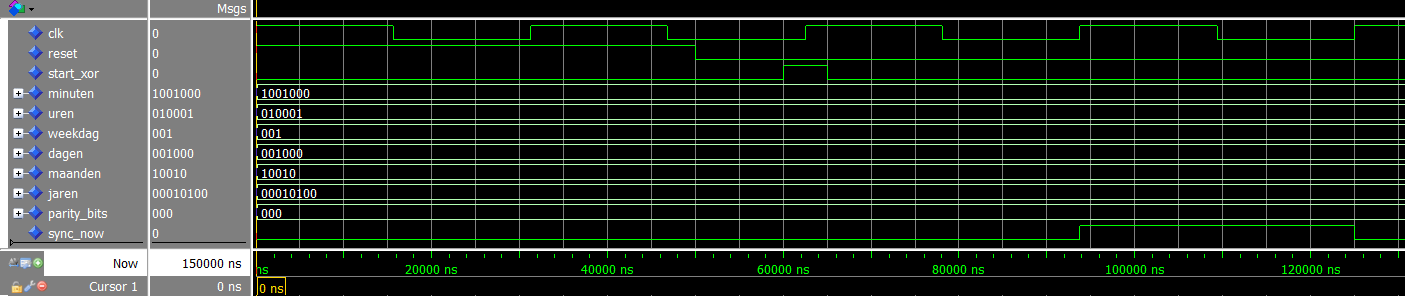
\includegraphics[width=\textwidth,height=\textheight,keepaspectratio]{Figuren/DCF77/Parity_check.png}
\caption{Simulatie van de parity check (150 microseconden)}
\end{figure}
\phantomsection\subsection*{\refstepcounter{subsection}\label{fig: synctime_beh}\thesubsection.\quad Behaviour synctime}
\begin{figure}[ht!]
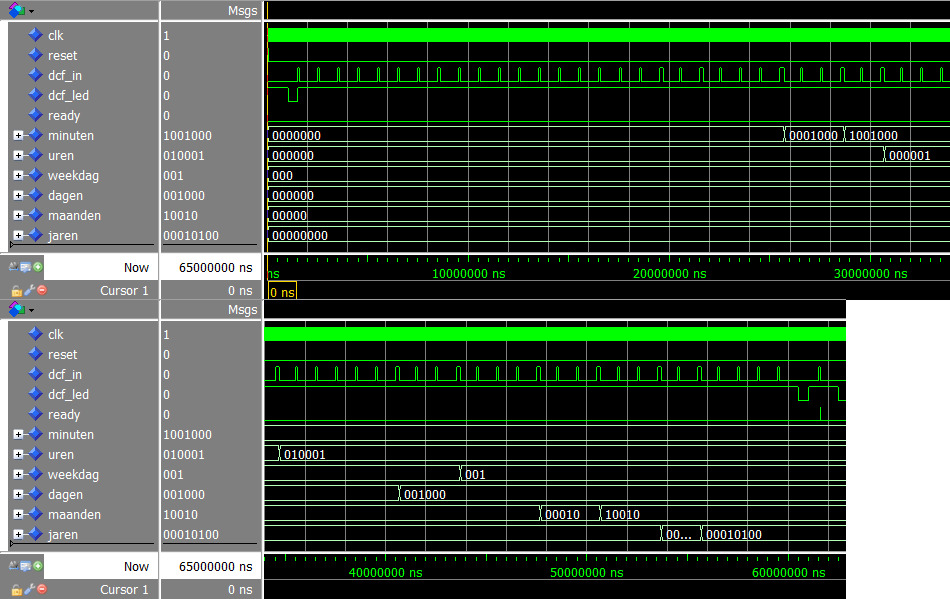
\includegraphics[width=\textwidth,height=\textheight,keepaspectratio]{Figuren/DCF77/Synctime.png}
\caption{Simulatie van synctime (65 ms op schaal)}
\end{figure}
\phantomsection\subsection*{\refstepcounter{subsection}\label{fig: klokdeler_beh}\thesubsection.\quad Behaviour klokdeler}
\begin{figure}[ht!]
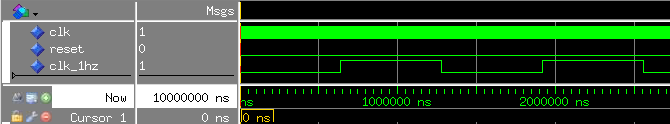
\includegraphics[width=\textwidth,height=\textheight,keepaspectratio]{Figuren/DCF77/Klokdeler.png}
\caption{Simulatie van de  klokdeler (10 ms op schaal)}
\end{figure}
\phantomsection\subsection*{\refstepcounter{subsection}\label{fig: mod24_beh}\thesubsection.\quad Behaviour mod24 teller}
\begin{figure}[ht!]
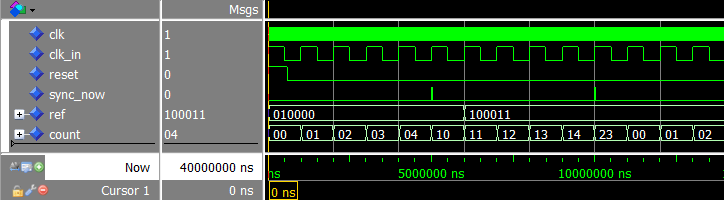
\includegraphics[width=\textwidth,height=\textheight,keepaspectratio]{Figuren/DCF77/Mod24_teller.png}
\caption{Simulatie van de mod24 teller (40 ms op schaal)}
\end{figure}
\phantomsection\subsection*{\refstepcounter{subsection}\label{fig: mod601_beh}\thesubsection.\quad Behaviour mod60 teller}
\begin{figure}[ht!]
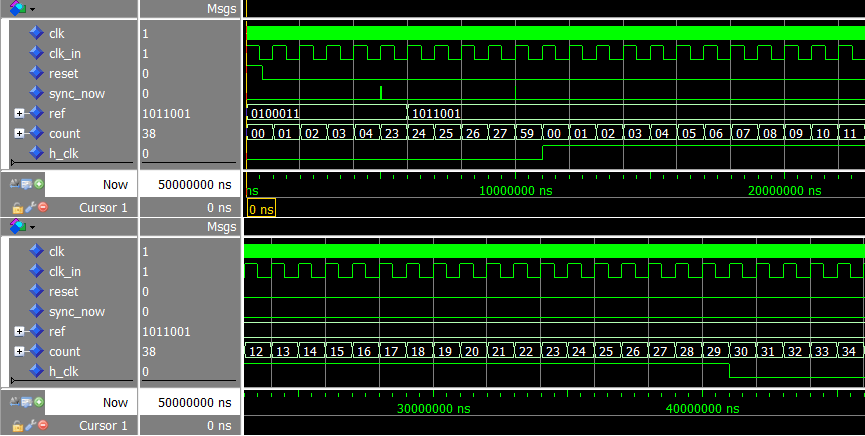
\includegraphics[width=\textwidth,height=\textheight,keepaspectratio]{Figuren/DCF77/Mod60_teller.png}
\caption{Simulatie van de mod60 teller (50 ms op schaal)}
\end{figure}
\phantomsection\subsection*{\refstepcounter{subsection}\label{fig: mod602_beh}\thesubsection.\quad Behaviour mod60 clock}
\begin{figure}[ht!]
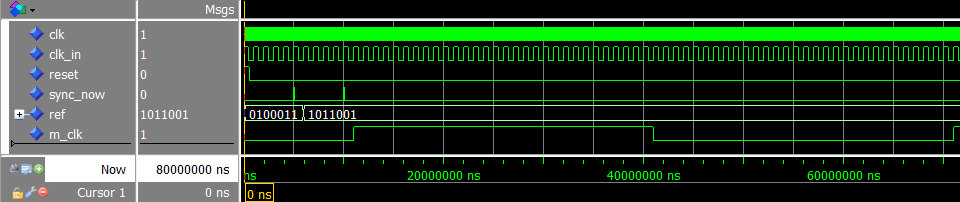
\includegraphics[width=\textwidth,height=\textheight,keepaspectratio]{Figuren/DCF77/Mod60_clock.png}
\caption{Simulatie van de mod60 clock (80 ms op schaal)}
\end{figure}
\phantomsection\subsection*{\refstepcounter{subsection}\label{fig: klok_beh}\thesubsection.\quad Behaviour klok}
\begin{figure}[ht!]
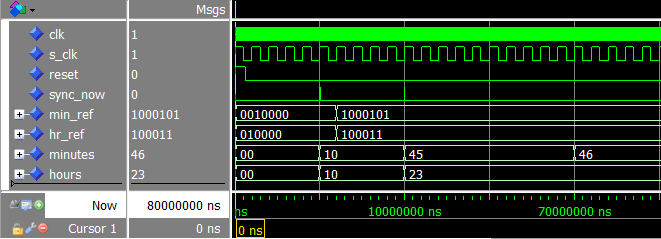
\includegraphics[width=\textwidth,height=\textheight,keepaspectratio]{Figuren/DCF77/Klok.png}
\caption{Simulatie van de klok (80 ms op schaal)}
\end{figure}
\phantomsection\subsection*{\refstepcounter{subsection}\label{fig: beh}\thesubsection.\quad Behaviour DCF77 blok}
\begin{figure}[ht!]
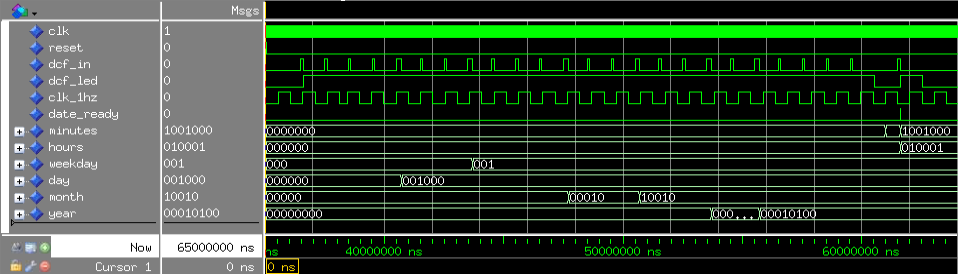
\includegraphics[width=\textwidth,height=\textheight,keepaspectratio]{Figuren/DCF77/Behaviour.png}
\caption{Simulatie van het DCF77 blok (65 ms op schaal)}
\end{figure}
\phantomsection\subsection*{\refstepcounter{subsection}\label{fig: switchlevel}\thesubsection.\quad Switch-level DCF77 blok}
\begin{figure}[ht!]
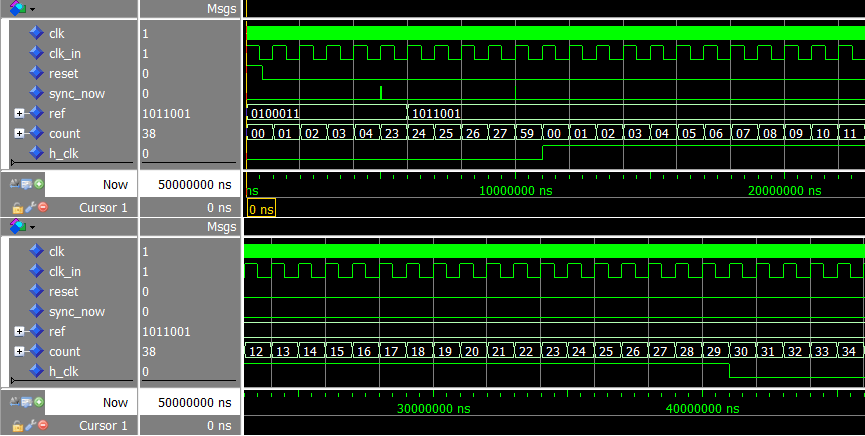
\includegraphics[width=\textwidth,height=\textheight,keepaspectratio]{Figuren/DCF77/Mod60_teller.png}
\caption{Switch-level simulatie van het DCF77 blok (65 ms op schaal)}
\end{figure}


\chapter[Simulatie resultaten]{Simulaties resultaten van de controller}
\label{Ap:sim_controller}
\section{Behavioral simulatie}
\begin{figure}[ht!]
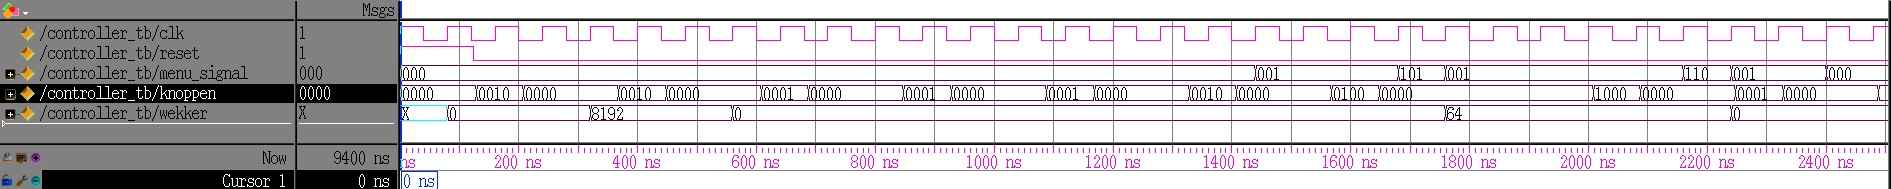
\includegraphics[width=\textwidth,height=\textheight,keepaspectratio]{Figuren/Controller/wave0-2_5_inv.jpg}
\caption{Simulatie van 0 tot 2500ns}
\label{fig:sim_beh_0-2_5}
\end{figure}
\begin{figure}[ht!]
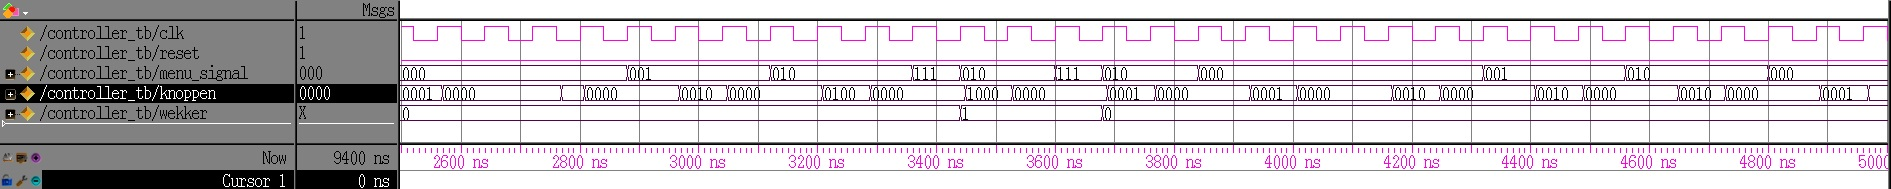
\includegraphics[width=\textwidth,height=\textheight,keepaspectratio]{Figuren/Controller/wave2_5-5_inv.jpg}
\caption{Simulatie van 2500ns tot 5000ns}
\label{fig:sim_beh_2_5-5}
\end{figure}
\begin{figure}[ht!]
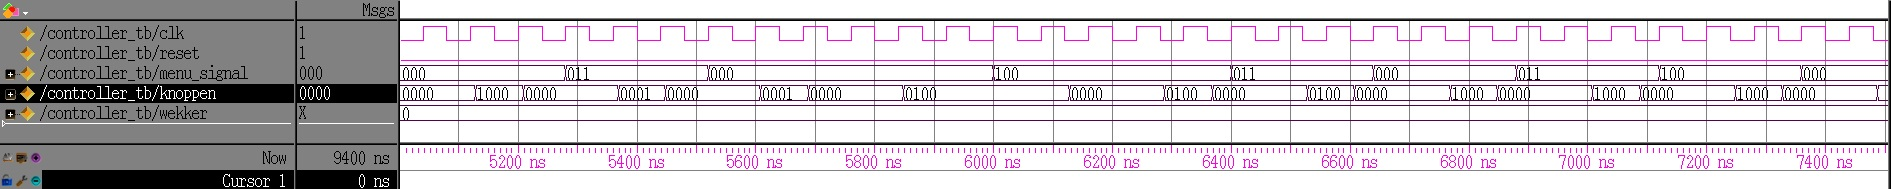
\includegraphics[width=\textwidth,height=\textheight,keepaspectratio]{Figuren/Controller/wave5-7_5_inv.jpg}
\caption{Simulatie van 5000ns tot 7500ns}
\label{fig:sim_beh_5-7_5}
\end{figure}
\begin{figure}[ht!]
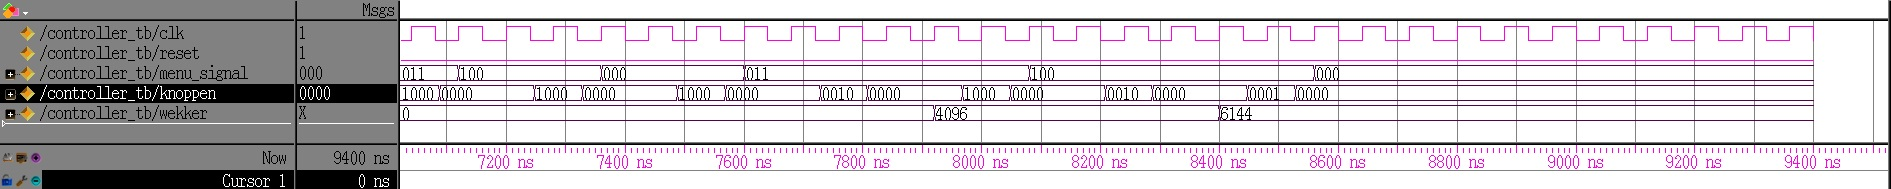
\includegraphics[width=\textwidth,height=\textheight,keepaspectratio]{Figuren/Controller/wave7_5-_inv.jpg}
\caption{Simulatie van 7500ns tot het einde}
\label{fig:sim_beh_7_5-}
\end{figure}
\newpage
\section{Synthesize simulatie}
\begin{figure}[ht!]
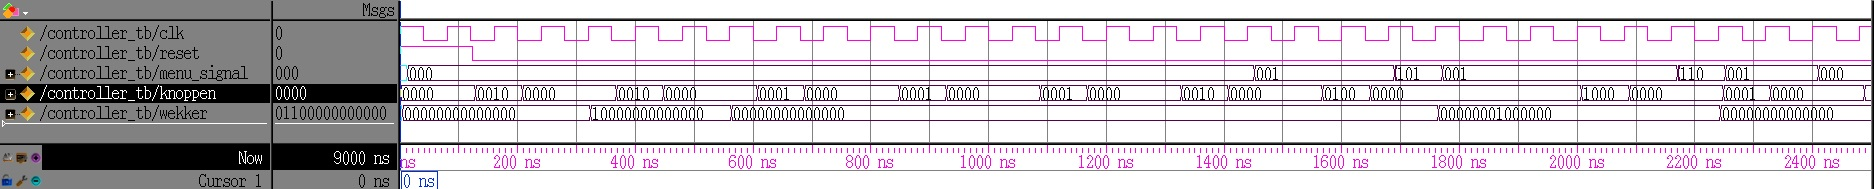
\includegraphics[width=\textwidth,height=\textheight,keepaspectratio]{Figuren/Controller/wave0-2_5_syn_inv.jpg}
\caption{Simulatie van 0 tot 2500ns}
\label{fig:sim_syn_0-2_5}
\end{figure}
\begin{figure}[ht!]
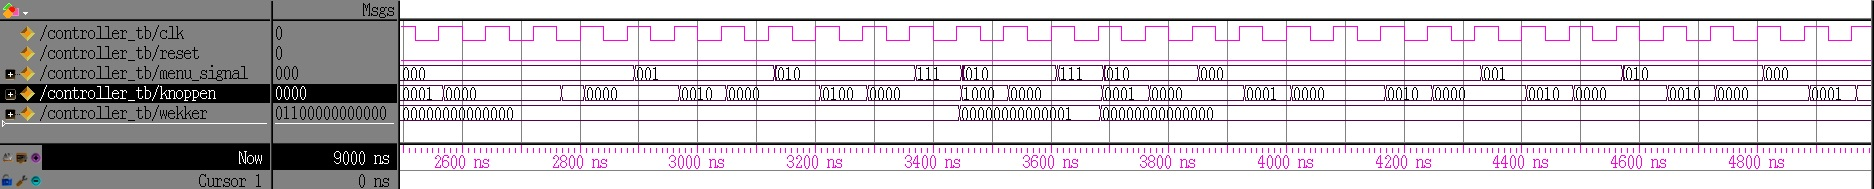
\includegraphics[width=\textwidth,height=\textheight,keepaspectratio]{Figuren/Controller/wave2_5-5_syn_inv.jpg}
\caption{Simulatie van 2500ns tot 5000ns}
\label{fig:sim_syn_2_5-5}
\end{figure}
\begin{figure}[ht!]
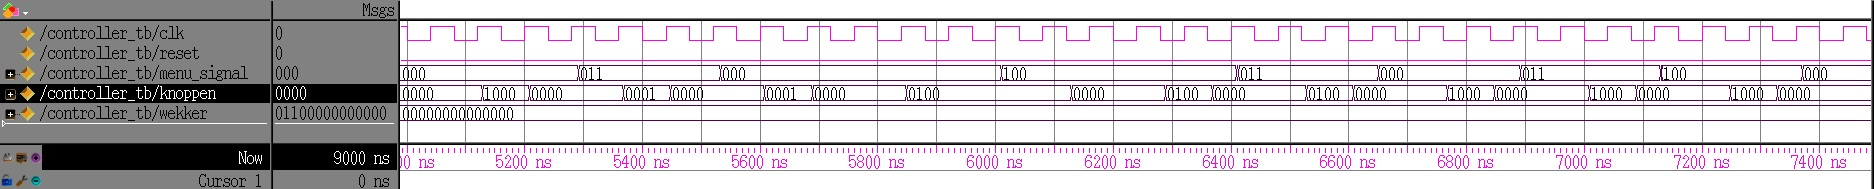
\includegraphics[width=\textwidth,height=\textheight,keepaspectratio]{Figuren/Controller/wave5-7_5_syn_inv.jpg}
\caption{Simulatie van 5000ns tot 7500ns}
\label{fig:sim_syn_5-7_5}
\end{figure}
\begin{figure}[ht!]
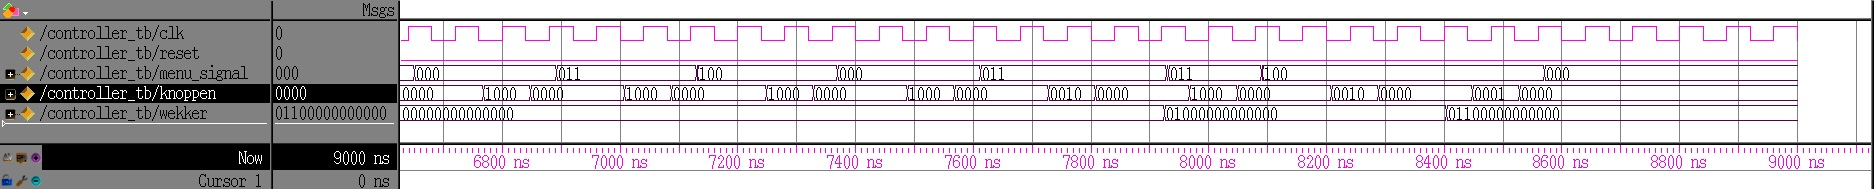
\includegraphics[width=\textwidth,height=\textheight,keepaspectratio]{Figuren/Controller/wave7_5-_syn_inv.jpg}
\caption{Simulatie van 7500ns tot het einde}
\label{fig:sim_syn_7_5-}
\end{figure}
\newpage
\section{Extracted simulatie}
\begin{figure}[ht!]
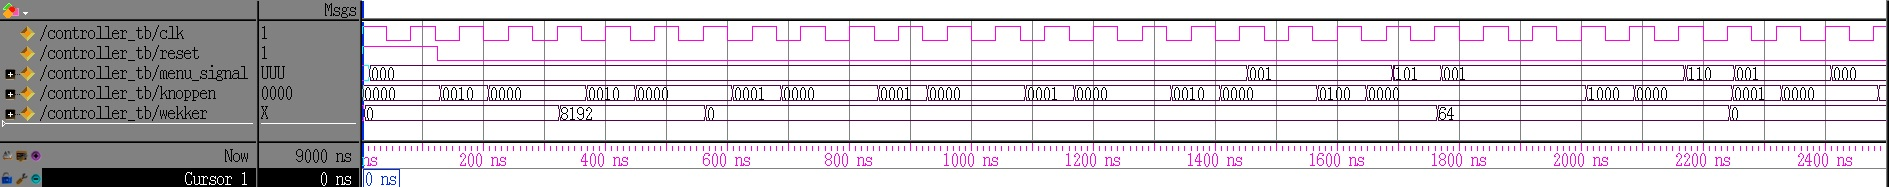
\includegraphics[width=\textwidth,height=\textheight,keepaspectratio]{Figuren/Controller/wave0-2_5_ext_inv.jpg}
\caption{Simulatie van 0 tot 2500ns}
\label{fig:sim_ext_0-2_5}
\end{figure}
\begin{figure}[ht!]
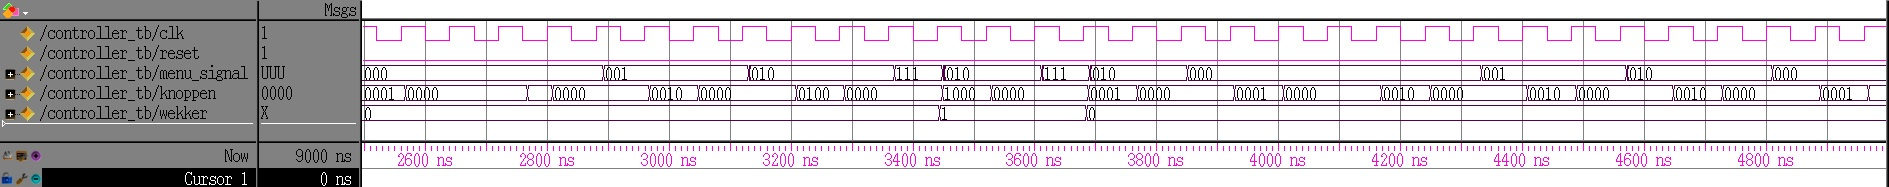
\includegraphics[width=\textwidth,height=\textheight,keepaspectratio]{Figuren/Controller/wave2_5-5_ext_inv.jpg}
\caption{Simulatie van 2500ns tot 5000ns}
\label{fig:sim_ext_2_5-5}
\end{figure}
\begin{figure}[ht!]
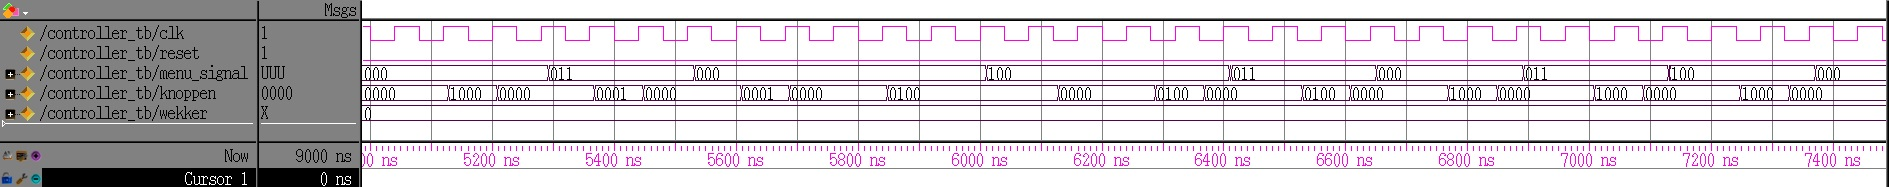
\includegraphics[width=\textwidth,height=\textheight,keepaspectratio]{Figuren/Controller/wave5-7_5_ext_inv.jpg}
\caption{Simulatie van 5000ns tot 7500ns}
\label{fig:sim_ext_5-7_5}
\end{figure}
\begin{figure}[ht!]
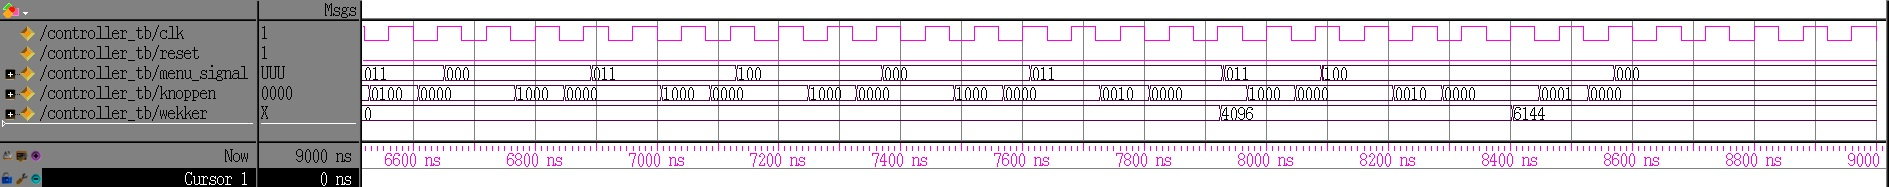
\includegraphics[width=\textwidth,height=\textheight,keepaspectratio]{Figuren/Controller/wave7_5-_ext_inv.jpg}
\caption{Simulatie van 7500ns tot het einde}
\label{fig:sim_ext_7_5-}
\end{figure}
\newpage
\section{Timing}
\begin{figure}[ht!]
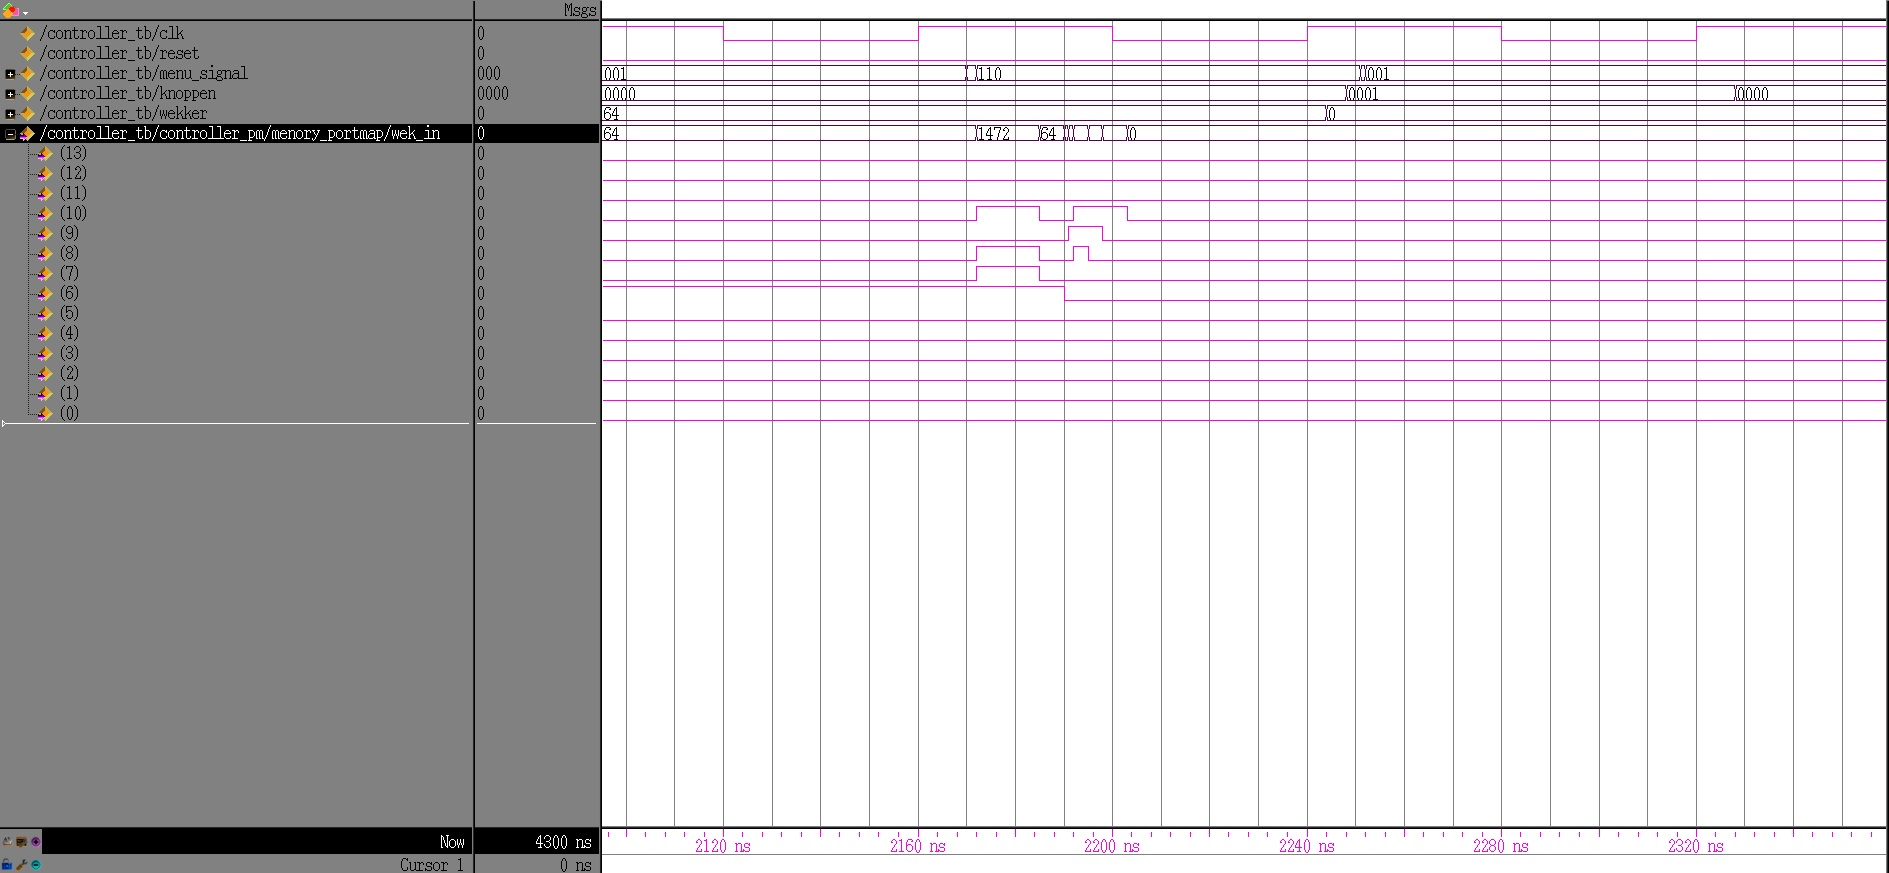
\includegraphics[width=\textwidth,height=\textheight,keepaspectratio]{Figuren/Controller/gliches_min_inv.jpg}
\caption{Timing problemen}
\label{fig:timing_controller}
\end{figure}

\chapter[Simulatie resultaten Alarm]{Simulaties resultaten van het alarm}
\label{Ap:sim_alarm}
\section{Behavioral simulatie}
\begin{figure}[ht!]
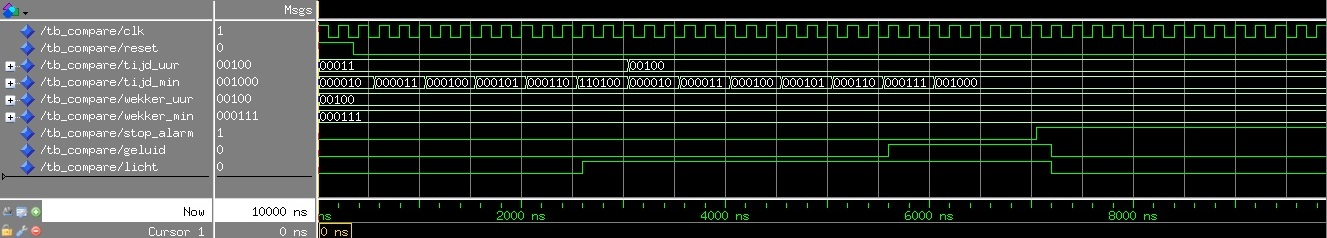
\includegraphics[width=\textwidth,height=\textheight,keepaspectratio]{Figuren/Alarm/Compare_beh.jpg}
\caption{Simulatie van 0 tot 10000 ns van compare}
\label{fig:sim_beh_compare}
\end{figure}
\begin{figure}[ht!]
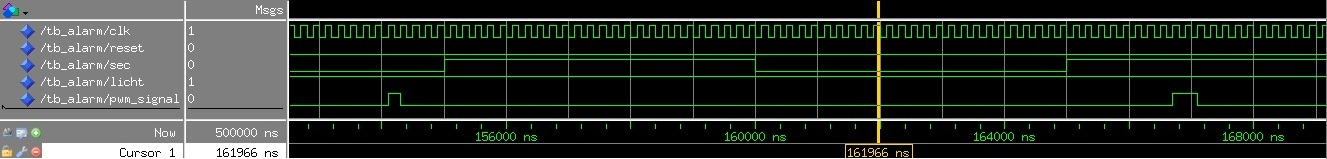
\includegraphics[width=\textwidth,height=\textheight,keepaspectratio]{Figuren/Alarm/Alarm_beh.jpg}
\caption{Simulatie van 151000 tot 170000 ns van alarm}
\label{fig:sim_beh_alarm}
\end{figure}
\newpage
\section{Extracted simulatie}
\begin{figure}[ht!]
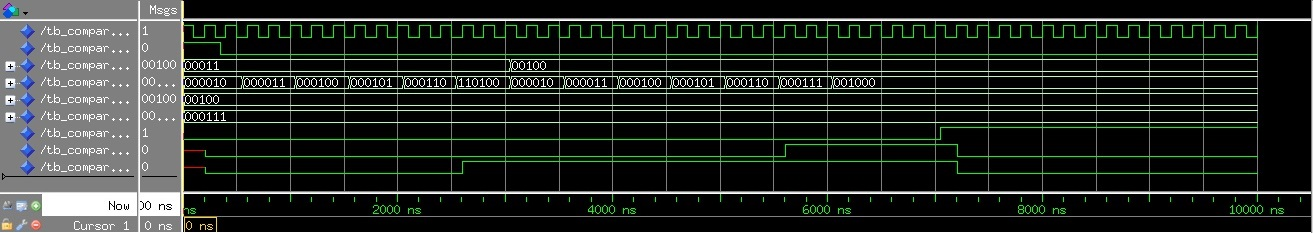
\includegraphics[width=\textwidth,height=\textheight,keepaspectratio]{Figuren/Alarm/Compare_ext.jpg}
\caption{Simulatie van 0 tot 10000 ns van alarm}
\label{fig:sim_ext_compare}
\end{figure}
\begin{figure}[ht!]
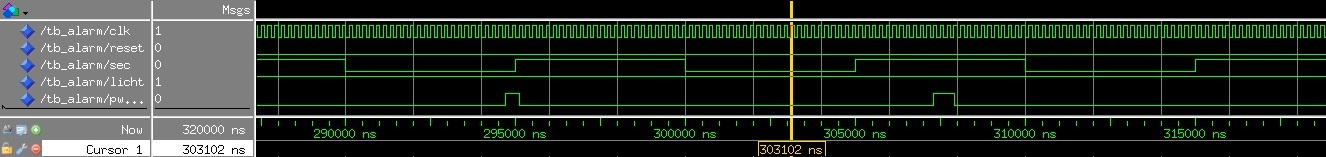
\includegraphics[width=\textwidth,height=\textheight,keepaspectratio]{Figuren/Alarm/Alarm_ext.jpg}
\caption{Simulatie van 290000 tot 320000 ns van alarm}
\label{fig:sim_ext_alarm}
\end{figure}

\chapter[Simulatie resultaten LCD]{Simulaties resultaten van het LCD}
\label{Ap:sim_LCD}
\section{Menu}
\begin{figure}[h!]
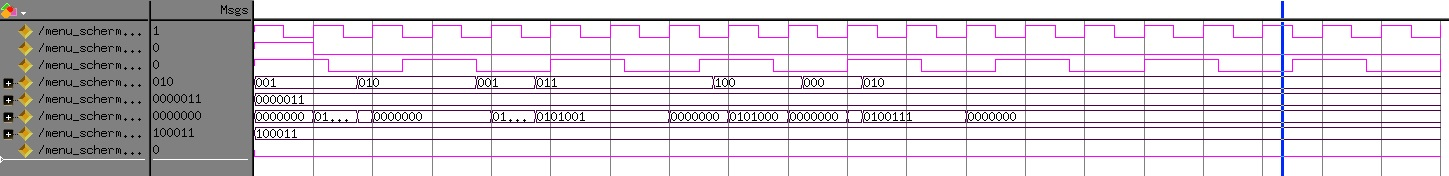
\includegraphics[width=\textwidth,height=\textheight,keepaspectratio]{Figuren/LCD/resultaten/menu.jpg}
\caption{Simulatie van het subblok menu}
\label{fig:simmenu}
\end{figure}
\section{Geluid}
\begin{figure}[h!]
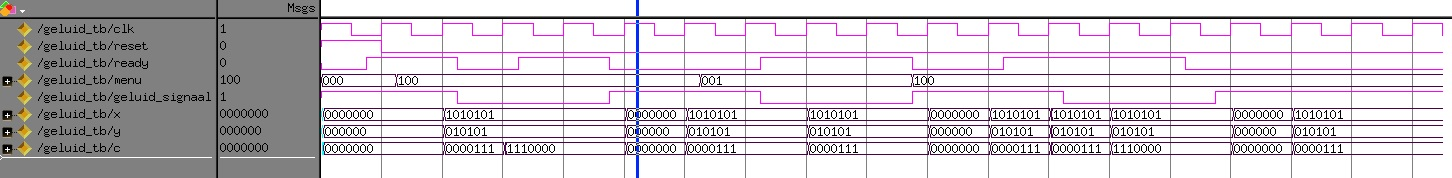
\includegraphics[width=\textwidth,height=\textheight,keepaspectratio]{Figuren/LCD/resultaten/geluid.jpg}
\caption{Simulatie van het subblok geluid}
\label{fig:simgeluid}
\end{figure}
\section{Licht}
\begin{figure}[h!]
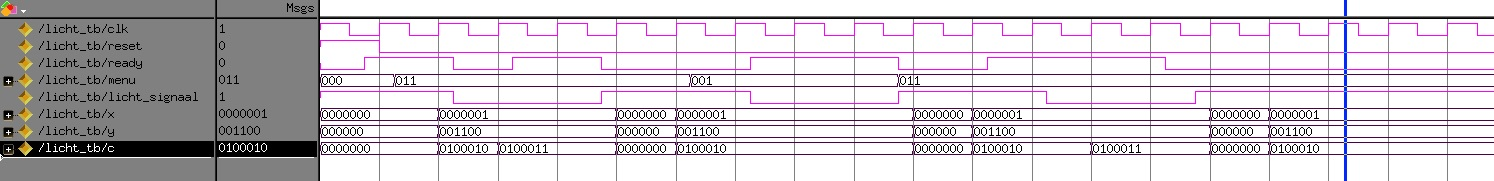
\includegraphics[width=\textwidth,height=\textheight,keepaspectratio]{Figuren/LCD/resultaten/licht.jpg}
\caption{Simulatie van het subblok licht}
\label{fig:simlicht}
\end{figure}
\section{DCF}
\begin{figure}[h!]
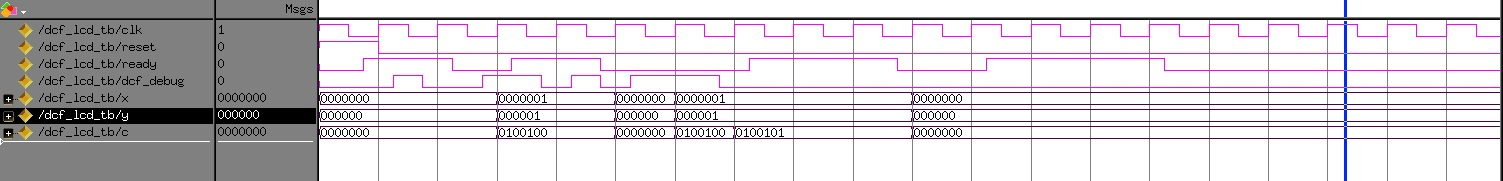
\includegraphics[width=\textwidth,height=\textheight,keepaspectratio]{Figuren/LCD/resultaten/dcf.jpg}
\caption{Simulatie van het subblok dcf}
\label{fig:simdcf}
\end{figure}

\begin{figure}[h!]
\includegraphics[width=\textwidth,height=\textheight,keepaspectratio]{Figuren/LCD/resultaten/simulatie_datum_behavioural.png}
\caption{Simulatie behavioural van het subblok datum}
\label{fig:sim_datum_behavioural}
\end{figure}

\begin{figure}[h!]
\includegraphics[width=\textwidth,height=\textheight,keepaspectratio]{Figuren/LCD/resultaten/simulatie_datum_circuit.png}
\caption{Simulatie circuit van het subblok datum}
\label{fig:sim_datum_circuit}
\end{figure}

\begin{figure}[h!]
	\includegraphics[width=\textwidth,height=\textheight,keepaspectratio]{Figuren/LCD/resultaten/sim_tijd.png}
	\caption{Simulatie van het subblok tijd}
	\label{fig:sim_tijd}
\end{figure}

\begin{figure}[h!]
	\includegraphics[width=\textwidth,height=\textheight,keepaspectratio]{Figuren/LCD/resultaten/sim_wektijd.png}
	\caption{Simulatie van het subblok wektijd}
	\label{fig:sim_wektijd}
\end{figure}

\begin{figure}[h!]
	\includegraphics[width=\textwidth,height=\textheight,keepaspectratio]{Figuren/LCD/resultaten/sim_send_top.png}
	\caption{Simulatie van de subblokken send controller en de send bus}
	\label{fig:sim_send_top}
\end{figure}
\bibliography{Referenties}

\end{document}